\ifx\pdfminorversion\undefined\else\pdfminorversion=4\fi
\documentclass[aspectratio=169,t, table]{beamer}
%\documentclass[aspectratio=169,t,handout]{beamer}

% English version FAU Logo
\usepackage[english]{babel}
% German version FAU Logo
%\usepackage[ngerman]{babel}

\usepackage[utf8]{inputenc}
\usepackage[sfdefault]{roboto}
\usepackage[T1]{fontenc}
\usepackage{amsmath,amssymb}
\usepackage{graphicx}
\usepackage{listings}
\usepackage[backend=biber,sorting=none,doi=true,style=ieee]{biblatex}

% Options:
%  - inst:      Institute
%                 med:      MedFak FAU theme
%                 nat:      NatFak FAU theme
%                 phil:     PhilFak FAU theme
%                 rw:       RWFak FAU theme
%                 rw-jura:  RWFak FB Jura FAU theme
%                 rw-wiso:  RWFak FB WISO FAU theme
%                 tf:       TechFak FAU theme
%  - image:     Cover image on title page
%  - plain:     Plain title page
%  - longtitle: Title page layout for long title
\usetheme[%
	image,%
	longtitle,%
	inst=tf%
]{fau}

% Enable semi-transparent animation preview
\setbeamercovered{transparent}

% Enable frame numbering
%\setbeamertemplate{footline}[frame number]


\lstset{%
	language=Python,
	tabsize=2,
	basicstyle=\tt,
	keywordstyle=\color{blue},
	commentstyle=\color{green!50!black},
	stringstyle=\color{red},
	numbers=left,
	numbersep=0.5em,
	xleftmargin=1em,
	numberstyle=\tt
}

\defbibheading{bibliography}{}
\addbibresource{references.bib}

\date[SS2023]{Summer semester 2023}


\usepackage{url}
\usepackage{hyperref}
\usepackage{fontawesome5}
\usepackage{graphicx}
\usepackage{booktabs}
\usepackage{calc}
\usepackage{ifthen}

\usepackage{tabularx}
\usepackage{longtable}
\usepackage{makecell}

\usepackage{xcolor}
\definecolor{airforceblue}{rgb}{0.36, 0.54, 0.66}
\definecolor{ForestGreen}{rgb}{0.34, 0.139, 0.34}

% English version
\institute[CS6]{Chair of Computer Science 6 (Data Management), Friedrich-Alexander University Erlangen-N\"urnberg}
% German version
% \institute[Lehrstuhl]{Lehrstuhl, Friedrich-Alexander-Universit\"at Erlangen-N\"urnberg}

\setbeamertemplate{section in toc}[sections numbered]

\setbeamertemplate{section page}{%
	\begingroup
	\begin{beamercolorbox}[sep=10pt,center,rounded=true,shadow=true]{section title}
		\usebeamerfont{section title}\thesection~\insertsection\par
	\end{beamercolorbox}
	\endgroup
}

\usepackage{tikz}
\usepackage{tikz-cd}
\usepackage{pgfplots,pgfplotstable,pgf-pie}

\newcommand{\tikzmark}[1]{\tikz[remember picture] \node[coordinate] (#1) {#1};}

\tikzset{
  every overlay node/.style={
    %draw=black,fill=white,rounded corners,
    anchor=north west, inner sep=0pt,
  },
}
% Usage:
% \tikzoverlay at (-1cm,-5cm) {content};
% or
% \tikzoverlay[text width=5cm] at (-1cm,-5cm) {content};
\def\tikzoverlay{%
   \tikz[remember picture, overlay]\node[every overlay node]
}%

\newcommand{\plots}{0.611201}
\newcommand{\plotm}{2.19882}

\newcommand{\MaxNumberX}{3}
\newcommand{\MaxNumberY}{5}

\pgfmathdeclarefunction{gauss}{2}{%
  \pgfmathparse{1/(#2*sqrt(2*pi))*exp(-((x-#1)^2)/(2*#2^2))}%
}

\tikzset{
  thick,
  >=latex,
  every edge/.style={draw=gray, thick, >=latex},
  vertex/.style = {
    circle,
    fill            = black,
    outer sep = 2pt,
    inner sep = 1pt,
  }
}
\usetikzlibrary{matrix,mindmap}
\usetikzlibrary{arrows,decorations.pathmorphing,backgrounds,fit,positioning,shapes.symbols,chains,intersections,snakes}
\tikzset{level 1/.append style={sibling angle=50,level distance = 165mm}}
\tikzset{level 2/.append style={sibling angle=20,level distance = 45mm}}
\tikzset{every node/.append style={scale=1}}
% read in data file
\pgfplotstableread{data/iris.dat}\iris
% get number of data points
\pgfplotstablegetrowsof{\iris}
\pgfmathsetmacro\NumRows{\pgfplotsretval-1}

\usepgfplotslibrary{groupplots}
\pgfplotsset{height=4cm,width=8cm,compat=1.14}

\tikzset{
    vertex/.style = {
        circle,
        fill            = black,
        outer sep = 2pt,
        inner sep = 1pt,
    }
}

\tikzset{
    mynode/.style={
        draw,
        thick,
        anchor=south west,
        minimum width=2cm,
        minimum height=1.3cm,
        align=center,
        inner sep=0.2cm,
        outer sep=0,
        rectangle split,
        rectangle split parts=2,
        rectangle split draw splits=false},
    reverseclip/.style={
        insert path={(current page.north east) --
            (current page.south east) --
            (current page.south west) --
            (current page.north west) --
            (current page.north east)}
    }
}

\tikzset{basic/.style={
        draw,
        rectangle split,
        rectangle split parts=2,
        rectangle split part fill={blue!20,white},
        minimum width=2.5cm,
        text width=2cm,
        align=left,
        font=\itshape
    },
    Diamond/.style={ diamond,
                      draw,
                      shape aspect=2,
                      inner sep = 2pt,
                      text centered,
                      fill=blue!10!white,
                      font=\itshape
                    }}


\tikzset{level 1/.append style={sibling angle=50,level distance = 165mm}}
\tikzset{level 2/.append style={sibling angle=20,level distance = 45mm}}
\tikzset{every node/.append style={scale=1}}

\usetikzlibrary{arrows,decorations.pathmorphing,backgrounds,fit,positioning,shapes.symbols,chains,intersections,snakes,positioning,matrix,mindmap,shapes.multipart,shapes,calc,shapes.geometric}


\usepackage{cleveref}
\newcommand*{\fullref}[1]{\underline{\hyperref[{#1}]{\cref{#1} (\nameref*{#1})}}}

\setbeamercovered{invisible}
\usepackage[linesnumbered]{algorithm2e}
\usepackage{multirow}
\usepackage{array}
\newcommand*\revealcline{\noalign{\vskip\arrayrulewidth}} % used in 5-evaluation-selection
% Title, authors, and date
\title[KDD~7.~Classification]{7. Classification} %
\subtitle{Knowledge Discovery in Databases}
\author[M.~B.~Sigl]{Melanie Bianca Sigl, \texttt{melanie.sigl@fau.de}}

\input{x-additional/vc.tex}

\hypersetup{
	pdfkeywords={},
	pdfsubject={Version \GITAbrHash},
	pdfcreator={},
	pdflang={English}
}



% Set additional logo (overwrites FAU seal)
%\logo{\includegraphics[width=.15\textwidth]{themefau/art/xxx/xxx.pdf}}
\begin{filecontents}{data.dat}
	2 0.0629921259843
	3 0.0236220472441
	4 0.0314960629921
	5 0.125984251969
	6 0.0629921259843
	7 0.102362204724
	8 0.110236220472
	9 0.0551181102362
	10 0.0629921259843
	11 0.0314960629921
	12 0.0236220472441
	13 0.0314960629921
	14 0.0629921259843
	15 0.0551181102362
	16 0.0393700787402
	17 0.0472440944882
	18 0.00787401574803
	19 0.0393700787402
	24 0.00787401574803
	27 0.00787401574803
	33 0.00787401574803
\end{filecontents}

\begin{document}
\pgfplotstableread{
10.46365192956
90.22330318663
15.4712651178
80.87219994452
90.92824632322
80.69935247007
170.8222081627
140.3601041144
220.9047131581
80.05005282649
90.650706465
170.2352199894
70.76424153088
10.370245979
70.12513239519
20.64730407495
70.2072208982
14.7683650153
14.0063750733
19.324137585
20.40858604381
18.0368674939
80.02681240716
80.26418810694
120.1941169594
90.62080674537
30.24961728242
30.27316960403
170.9038479307
70.40481579419
10.814441695
80.40741573499
60.08031313304
130.1781459953
100.206134367
150.0864695726
90.03013313987
40.46906993699
90.27542593922
110.387166818
50.34088290758
70.35790199406
110.8693581818
100.8557924873
130.969617244
100.6354692297
30.03046442179
60.60358722529
120.2836888554
80.46665782108
130.9221860476
150.1323993544
70.16507829073
50.69317421704
150.4624253296
160.9138444234
60.44259653768
160.4478862876
30.46926929558
100.8862152053
100.4982459647
130.079580222
100.8219448481
120.1887774019
20.27608579327
40.21879129366
80.6626149873
30.05616084556
120.2628717929
30.07385860151
120.1834370192
70.86785100457
220.3039915506
70.6084726129
30.38040559575
40.77264935147
130.9493967532
140.1237678197
60.79956429934
80.7032357113
60.08645967617
90.19491098171
17.1651582777
40.7041931405
30.78091331321
50.20247821499
13.8921717364
60.09560236506
18.5811121283
10.3758110312
80.95955605147
12.4511725524
40.67834498484
11.0234433275
15.364443589
80.23928346825
60.30079928878
90.95330967273
12.5692010856
11.8362767596
}\datatable
\pgfplotstablesort{\sorted}{\datatable}
\pgfplotstablegetrowsof{\datatable}
\edef\numrows{\pgfplotsretval}

% Title
\maketitle

{ % Outline
	\setbeamertemplate{footline}{}
	\begin{frame}[noframenumbering]{Outline}
		\tableofcontents

	\end{frame}
}

% Body
\section{Basic Concepts}

\begin{frame}{What is Cluster Analysis?}
	\begin{itemize}
		\item \textbf{{\color{airforceblue}Cluster}: A collection of data 
		objects within a larger set that are:}
		\begin{itemize}
			\item {\color{airforceblue}Similar (or related)} to one another 
			within the same group and,
			\item dissimilar (or unrelated) to the objects outside the group.
		\end{itemize}
		\item \textbf{{\color{airforceblue}Cluster analysis} (or clustering, 
		data segmentation, $\ldots$):}
		\begin{itemize}
			\item {\color{airforceblue}Define similarities} among data based on 
			the characteristics found in the data (input from user!).
			\item Group similar data objects into clusters.
		\end{itemize}
		\item \textbf{Unsupervised learning:}
		\begin{itemize}
			\item No predefined classes.
			\item I.e., learning by observation (vs. learning by examples: 
			supervised).
		\end{itemize}
		\item \textbf{Typical applications:}
		\begin{itemize}
			\item As a stand-alone tool to get insight into data distribution.
			\item As a preprocessing step for other algorithms.
		\end{itemize}
	\end{itemize}
\end{frame}

\begin{frame}{Clustering for Data Understanding and Applications}
	\begin{itemize}
		\item \textbf{Biology:}
		\begin{itemize}
			\item Taxonomy of living things: kingdom, phylum, class, order, 
			family, genus, and species.
		\end{itemize}
		\item \textbf{Land use:}
		\begin{itemize}
			\item Identification of areas of similar land use in an 
			earth-observation database.
		\end{itemize}
		\item \textbf{Marketing:}
		\begin{itemize}
			\item Help marketers discover distinct groups in their customer 
			bases, and then use this knowledge to develop targeted marketing 
			programs.
		\end{itemize}
		\item \textbf{City planning:}
		\begin{itemize}
			\item Identifying groups of houses according to their house type, 
			value, and geographical location.
		\end{itemize}
		\item \textbf{Earthquake studies:}
		\begin{itemize}
			\item Observed earthquake epicenters should be clustered along 
			continent faults.
		\end{itemize}
		\item \textbf{Climate:}
		\begin{itemize}
			\item Understanding earth climate, find patterns of atmosphere and 
			ocean.
		\end{itemize}
	\end{itemize}
\end{frame}

\begin{frame}{Quality: What is Good Clustering?}
	\begin{itemize}
		\item \textbf{A good clustering method will produce high-quality 
		clusters.}
		\begin{itemize}
			\item \textbf{\color{airforceblue}High intra-class similarity:}
			\begin{itemize}
				\item Cohesive within clusters.
			\end{itemize}
			\item \textbf{\color{airforceblue}Low inter-class similarity:}
			\begin{itemize}
				\item Distinctive between clusters.
			\end{itemize}
		\end{itemize}
		\item \textbf{The {\color{airforceblue}quality} of a clustering method 
		depends on:}
		\begin{itemize}
			\item the \textbf{\color{airforceblue}similarity measure} used by 
			the method,
			\item its implementation, and
			\item its ability to discover some or all of the hidden patterns.
		\end{itemize}
	\end{itemize}
\end{frame}

\begin{frame}{Measure the Quality of Clustering}
	\begin{itemize}
		\item \textbf{Dissimilarity/similarity metric:}
		\begin{itemize}
			\item Similarity is expressed in terms of a distance function, 
			typically a metric: $d(x,y)$.
			\item The definitions of distance functions are usually rather 
			different for interval-scaled, boolean, categorical, ordinal, 
			ratio, and vector variables (see chapter 2).
			\item \textbf{\color{airforceblue}Weights} should be associated 
			with different variables \\
			based on applications and data semantics.
		\end{itemize}
		\item \textbf{Quality of clustering:}
		\begin{itemize}
			\item There is usually a separate 
			\textbf{\color{airforceblue}"quality" function} that measures the 
			"goodness" of a cluster.
			\item It is hard to define "similar enough" or "good enough."
			\item The answer is typically highly subjective.
		\end{itemize}
	\end{itemize}
\end{frame}

\begin{frame}{Considerations for Cluster Analysis}
	\begin{itemize}
		\item \textbf{Partitioning criteria:}
		\begin{itemize}
			\item Single level vs. hierarchical partitioning.
			\item Often, multi-level hierarchical partitioning is desirable.
		\end{itemize}
		\item \textbf{Separation of clusters:}
		\begin{itemize}
			\item Exclusive (e.g., one customer belongs to only one region) vs.
			\item Non-exclusive (e.g., one document may belong to more than one 
			class).
		\end{itemize}
		\item \textbf{Similarity measure:}
		\begin{itemize}
			\item Distance-based (e.g., Euclidean, road network, vector) vs.
			\item Connectivity-based (e.g., density or contiguity).
		\end{itemize}
		\item \textbf{Clustering space:}
		\begin{itemize}
			\item Full space (often when low-dimensional) vs.
			\item Subspaces (often in high-dimensional clustering).
		\end{itemize}
	\end{itemize}
\end{frame}

\begin{frame}{Requirements and Challenges}
	\begin{itemize}
		\item \textbf{Scalability:}
		\begin{itemize}
			\item Clustering all the data instead of only the samples.
		\end{itemize}
		\item \textbf{Ability to deal with different types of attributes:}
		\begin{itemize}
			\item Numerical, binary, categorical, ordinal, linked, and mixture 
			of these.
		\end{itemize}
		\item \textbf{Constraint-based clustering:}
		\begin{itemize}
			\item User may give inputs on constraints.
			\item Use domain knowledge to determine input parameters.
		\end{itemize}
		\item \textbf{Interpretability and usability.}
		\item \textbf{Others:}
		\begin{itemize}
			\item Discovery of clusters with arbitrary shape.
			\item Ability to deal with noisy data.
			\item Incremental clustering and insensitivity to input order.
			\item High dimensionality.
		\end{itemize}
	\end{itemize}
\end{frame}

\begin{frame}{Major Clustering Approaches}
	\begin{itemize}
		\item \textbf{Partitioning approach:}
		\begin{itemize}
			\item Construct various partitions and then evaluate them by some 
			criterion.
			\item E.g., minimizing the sum of square errors.
			\item Typical methods: k-means, k-medoids, CLARA, CLARANS.
		\end{itemize}
		\item \textbf{Hierarchical approach:}
		\begin{itemize}
			\item Create a hierarchical decomposition of the set of data (or 
			objects) using some criterion.
			\item Typical methods: AGNES, DIANA, BIRCH, CHAMELEON.
		\end{itemize}
		\item \textbf{Density-based approach:}
		\begin{itemize}
			\item Based on connectivity and density functions.
			\item Typical methods: DBSCAN, OPTICS, DENCLUE.
		\end{itemize}
		\item \textbf{Grid-based approach:}
		\begin{itemize}
			\item Based on a multiple-level granularity structure.
			\item Typical methods: STING, WaveCluster, CLIQUE.
		\end{itemize}
	\end{itemize}
\end{frame}

\begin{frame}{Major Clustering Approaches (II)}
	\begin{itemize}
		\item \textbf{Model-based approach:}
		\begin{itemize}
			\item A model is hypothesized for each of the clusters and tries to 
			find the best fit of that model to each other.
			\item Typical methods: EM, SOM, COBWEB.
		\end{itemize}
		\item \textbf{Frequent-pattern-based approach:}
		\begin{itemize}
			\item Based on the analysis of frequent patterns.
			\item Typical methods: p-Cluster.
		\end{itemize}
		\item \textbf{User-guided or constraint-based approach:}
		\begin{itemize}
			\item Clustering by considering user-specified or 
			application-specific constraints.
			\item Typical methods: COD (obstacles), constrained clustering.
		\end{itemize}
		\item \textbf{Link-based clustering:}
		\begin{itemize}
			\item Objects are often linked together in various ways.
			\item Massive links can be used to cluster objects: SimRank, 
			LinkClus.
		\end{itemize}
	\end{itemize}
\end{frame}
\section{Decision-Tree Induction}

\begin{frame}{Decision-tree Induction: An Example}
	\begin{columns}
		\begin{column}{0.38\textwidth}
			\vspace{-3cm}
			\begin{itemize}
				\item \textbf{Training dataset: buys\_computer.}
				      \begin{itemize}
					      \item The dataset follows an example of Quinlan's ID3 (playing tennis).
				      \end{itemize}
				\item \textbf{Resulting tree:}\\[0.1cm]
			\end{itemize}
			\centering
			\begin{tikzpicture}
	\node[rounded corners=.25em,draw, fill=faugray!62] at (0,0) (a) {age?};
	\node[rounded corners=.25em,draw] at (-1.5,-0.7) (b) {<=30};
	\node[rounded corners=.25em,draw] at (0,-0.7) (c) {$31\ldots40$};
	\node[rounded corners=.25em,draw] at (1.5,-0.7) (d) {$>40$};
	\node[rounded corners=.25em,draw, fill=faugray!62] at (-1.5,-1.4) (e) {student?};
	\node[rounded corners=.25em,draw] at (-2,-2.1) (eno1) {no};
	\node[rounded corners=.25em,draw] at (-1,-2.1) (eyes1) {yes};
	\node[text=faured] at (-2,-2.8) (eno2) {no};
	\node[text=faugreen] at (-1,-2.8) (eyes2) {yes};
	\node[rounded corners=.25em,draw,fill=faugray!62] at (1.5,-1.4) (g) {credit rating?};
	\node[rounded corners=.25em,draw] at (2.2,-2.1) (gf) {fair};
	\node[rounded corners=.25em,draw] at (1,-2.1) (gex) {excellent};
	\node[text=faured] at (1,-2.8) (gno) {no};
	\node[text=faugreen] at (2.2,-2.8) (gyes) {yes};
	\node[text=faugreen] at (0,-2.8) (f) {yes};

	\draw (a)--(b);
	\draw (a)--(c);
	\draw (a)--(d);
	\draw (b)--(e);
	\draw (c)--(f);
	\draw (d)--(g);
	\draw (e)--(eno1);
	\draw (e)--(eyes1);
	\draw (eno1)--(eno2);
	\draw (eyes1)--(eyes2);
	\draw (g)--(gex);
	\draw (g)--(gf);
	\draw (gex)--(gno);
	\draw (gf)--(gyes);
\end{tikzpicture}

		\end{column}
		\begin{column}{0.62\textwidth}
			\small
			\begin{tabular}{|l|l|c|c|c|}
	\hline
	\rowcolor{faugray!62}\textbf{age} & \textbf{income} & \textbf{student} & \textbf{credit\_rating} & \textbf{buys\_computer} \\\hline
	$\leq 30$                         & high            & no               & fair                    & {\color{faured}no}      \\\hline
	$\leq 30$                         & high            & no               & excellent               & {\color{faured}no}      \\\hline
	$31\ldots40$                      & high            & no               & fair                    & {\color{faugreen}yes}   \\\hline
	$>40$                             & medium          & no               & fair                    & {\color{faugreen}yes}   \\\hline
	$>40$                             & low             & yes              & fair                    & {\color{faugreen}yes}   \\\hline
	$>40$                             & low             & yes              & excellent               & {\color{faured}no}      \\\hline
	$31\ldots40$                      & low             & yes              & excellent               & {\color{faugreen}yes}   \\\hline
	$\leq 30$                         & medium          & no               & fair                    & {\color{faured}no}      \\\hline
	$\leq 30$                         & low             & yes              & fair                    & {\color{faugreen}yes}   \\\hline
	$>40$                             & medium          & yes              & fair                    & {\color{faugreen}yes}   \\\hline
	$\leq 30$                         & medium          & yes              & excellent               & {\color{faugreen}yes}   \\\hline
	$31\ldots40$                      & medium          & no               & excellent               & {\color{faugreen}yes}   \\\hline
	$31\ldots40$                      & high            & yes              & fair                    & {\color{faugreen}yes}   \\\hline
	$>40$                             & medium          & no               & excellent               & {\color{faured}no}      \\\hline
\end{tabular}

		\end{column}
	\end{columns}
\end{frame}


\begin{frame}{Decision-tree Induction: An Example}
	\begin{columns}[t]
		\begin{column}{0.45\textwidth}
			\begin{figure}[h]
				\centering
				\begin{tikzpicture}
	\node[rounded corners=.25em,draw, fill=faugray!62] at (0,0) (a) {age?};
	\node[rounded corners=.25em,draw] at (-1.5,-0.7) (b) {<=30};
	\node[rounded corners=.25em,draw] at (0,-0.7) (c) {$31\ldots40$};
	\node[rounded corners=.25em,draw] at (1.5,-0.7) (d) {$>40$};
	\node[rounded corners=.25em,draw, fill=faugray!62] at (-1.5,-1.4) (e) {student?};
	\node[rounded corners=.25em,draw] at (-2,-2.1) (eno1) {no};
	\node[rounded corners=.25em,draw] at (-1,-2.1) (eyes1) {yes};
	\node[text=faured] at (-2,-2.8) (eno2) {no};
	\node[text=faugreen] at (-1,-2.8) (eyes2) {yes};
	\node[rounded corners=.25em,draw,fill=faugray!62] at (1.5,-1.4) (g) {credit rating?};
	\node[rounded corners=.25em,draw] at (2.2,-2.1) (gf) {fair};
	\node[rounded corners=.25em,draw] at (1,-2.1) (gex) {excellent};
	\node[text=faured] at (1,-2.8) (gno) {no};
	\node[text=faugreen] at (2.2,-2.8) (gyes) {yes};
	\node[text=faugreen] at (0,-2.8) (f) {yes};

	\draw (a)--(b);
	\draw (a)--(c);
	\draw (a)--(d);
	\draw (b)--(e);
	\draw (c)--(f);
	\draw (d)--(g);
	\draw (e)--(eno1);
	\draw (e)--(eyes1);
	\draw (eno1)--(eno2);
	\draw (eyes1)--(eyes2);
	\draw (g)--(gex);
	\draw (g)--(gf);
	\draw (gex)--(gno);
	\draw (gf)--(gyes);
\end{tikzpicture}

			\end{figure}

		\end{column}
		\begin{column}{0.55\textwidth}
			\textbf{Components of a decision tree}
			\begin{itemize}
				\item \tikzmark{root} \textbf{Root}: topmost node.
				\item \tikzmark{internal} \textbf{Internal node}: test on an attribute.
				\item \tikzmark{leaf-node} \textbf{Leaf node}: holds a class label, also called \textit{terminal node}.
				\item \tikzmark{branch} \textbf{Branch}: outcome of a leaf node's test coupled with a text. In this example: \texttt{excellent}.
			\end{itemize}
		\end{column}
	\end{columns}

	\begin{tikzpicture}[remember picture,overlay]
		\draw[faucyan,thick,->] ([yshift=1.5mm,xshift=-4mm]root) to[out=170,in=0] (age.east);
		\draw[faucyan,thick,->] ([yshift=1.5mm,xshift=-4mm]internal) to[out=180,in=10] (credit-rating.east);
		\draw[faucyan,thick,->] ([yshift=1.5mm,xshift=-4mm]leaf-node) to[out=190,in=30] (credit-yes.east);
		\draw[faucyan,thick,->] ([,xshift=-2.6mm]branch) to[out=-90,in=-90] ([xshift=1mm]$(credit-no.north east) + (.1em,.7em));
	\end{tikzpicture}
\end{frame}



\begin{frame}{Algorithm for Decision-tree Induction}
	\begin{itemize}
		\item \textbf{Basic algorithm (a greedy algorithm):}
		      \begin{itemize}
			      \item Tree is constructed in a \textbf{\color{airforceblue}top-down recursive divide-and-conquer manner.}
			      \item Attributes are categorical.
			            \begin{itemize}
				            \item If not: discretize in advance.
			            \end{itemize}
			      \item At start, all the training examples are at the root.
			      \item Examples are \textbf{\color{airforceblue}partitioned recursively} based on selected attributes.
			      \item Test attributes are selected on the basis of a heuristic or statistical measure.
			            \begin{itemize}
				            \item E.g., information gain -- see on the next slide.
			            \end{itemize}
		      \end{itemize}
		\item \textbf{Conditions for stopping partitioning:}
		      \begin{itemize}
			      \item All samples for a given node belong to the same class.
			      \item There are no remaining attributes for further partitioning.
			            \begin{itemize}
				            \item Majority voting is employed for classifying the leaf.
			            \end{itemize}
			      \item There are no samples left (i.e. partition for particular value is empty).
		      \end{itemize}
	\end{itemize}
\end{frame}

\begin{frame}{Attribute-selection Measure: Information Gain (ID3/C4.5)}
	\textbf{Select the attribute with the highest information gain.}
	\begin{itemize}
		\item Let $p_i$ be the probability that an arbitrary tuple in $D$ belongs to class $C_i$,\\ estimated by $\frac{|C_i|}{|D|}$, such that $1 \leq i \leq m$.
		\item \textbf{Expected information} (entropy) needed to classify a tuple in $D$:
		      \begin{align}
			      \text{Info}(D) = -\sum_{i=1}^{m}p_i \log_2(p_i).
		      \end{align}
		\item \textbf{Information} needed (after using attribute $A$ to split $D$ into $v$ partitions) to classify $D$:
		      \begin{align}
			      \text{Info}_A(D) = \sum_{j=1}^v \left( \frac{|D_j|}{|D|} \text{Info}(D_j) \right).
		      \end{align}
		\item \textbf{Information gained} by branching on $A$:
		      \begin{align}
			      \text{Gain}(A)=\text{Info}(D)-\text{Info}_A(D).
		      \end{align}
	\end{itemize}
\end{frame}

\begin{frame}{Attribute Selection: Information Gain}
	\begin{columns}
		\begin{column}{0.45\textwidth}
			\begin{itemize}
				\item \textbf{Class P: buys\_computer = "yes"}
				\item \textbf{Class N: buys\_computer = "no"}
				      \begin{align*}
					      \resizebox{7cm}{!}{%
						      $\text{Info}(D) = I(9,5) = - \frac{9}{14}\log_2(\frac{9}{14})-\frac{5}{14} \log_2(\frac{5}{14}) = 0.94$
					      }
				      \end{align*}
			\end{itemize}
			\centering
			\begin{tabular}{|l|l|l|l|}
				\hline
				\cellcolor{faugray!62}age     & \cellcolor{faugray!62}p & \cellcolor{faugray!62}n & \cellcolor{faugray!62}$l(p,n)$ \\\hline
				\cellcolor{white}$\leq 30$    & 2                       & 3                       & 0.971                          \\\hline
				\cellcolor{white}$31\ldots40$ & 4                       & 0                       & 0                              \\\hline
				\cellcolor{white}$>40$        & 3                       & 2                       & 0.971                          \\\hline
			\end{tabular}\\[0.2cm]
			\begin{itemize}
				\item \textbf{Similarly,}
				      \begin{itemize}
					      \item $\text{Gain}(\texttt{income}) = 0.029$,
					      \item $\text{Gain}(\texttt{student}) = 0.090$,
					      \item $\text{Gain}(\texttt{credit\_rating}) = 0.048$.
				      \end{itemize}
			\end{itemize}
		\end{column}
		\begin{column}{0.45\textwidth}
			\vspace{-1.3cm}
			\begin{align*}
				\resizebox{7cm}{!}{%
				$\text{Info}_{\texttt{age}}(D) = \frac{5}{14}I(2,3) + \frac{4}{14} I(4,0) + \frac{5}{14} I(3,2) = 0.694$.
				}
			\end{align*}
			$\frac{5}{14} I(2,3)$ means "$\texttt{age} \leq 30$" has $5$ out of $14$ samples, with $2$ yes'es and $3$ no's. Hence,
			\begin{align*}
				\text{Gain}(\texttt{age}) = \text{Info}(D)-\text{Info}_{\texttt{age}}(D) = 0.246.
			\end{align*}

			\resizebox{6cm}{!}{%
				\centering
				\begin{tabular}{|l|l|c|c|c|}
	\hline
	\rowcolor{faugray!62}\textbf{age} & \textbf{income} & \textbf{student} & \textbf{credit\_rating} & \textbf{buys\_computer} \\\hline
	$\leq 30$                         & high            & no               & fair                    & {\color{faured}no}      \\\hline
	$\leq 30$                         & high            & no               & excellent               & {\color{faured}no}      \\\hline
	$31\ldots40$                      & high            & no               & fair                    & {\color{faugreen}yes}   \\\hline
	$>40$                             & medium          & no               & fair                    & {\color{faugreen}yes}   \\\hline
	$>40$                             & low             & yes              & fair                    & {\color{faugreen}yes}   \\\hline
	$>40$                             & low             & yes              & excellent               & {\color{faured}no}      \\\hline
	$31\ldots40$                      & low             & yes              & excellent               & {\color{faugreen}yes}   \\\hline
	$\leq 30$                         & medium          & no               & fair                    & {\color{faured}no}      \\\hline
	$\leq 30$                         & low             & yes              & fair                    & {\color{faugreen}yes}   \\\hline
	$>40$                             & medium          & yes              & fair                    & {\color{faugreen}yes}   \\\hline
	$\leq 30$                         & medium          & yes              & excellent               & {\color{faugreen}yes}   \\\hline
	$31\ldots40$                      & medium          & no               & excellent               & {\color{faugreen}yes}   \\\hline
	$31\ldots40$                      & high            & yes              & fair                    & {\color{faugreen}yes}   \\\hline
	$>40$                             & medium          & no               & excellent               & {\color{faured}no}      \\\hline
\end{tabular}

			}
		\end{column}
	\end{columns}
\end{frame}

\begin{frame}{Partitioning in the Example}
	\centering
	\begin{tikzpicture}
		\node[rounded corners=0.25em,draw, fill=faugray!62] at (0,0) (r) {age?};
		\node[rounded corners=0.25em,draw] at (-2,-1) (a) {$\leq 30$};
		\node[rounded corners=0.25em,draw] at (0,-1) (b) {$31\ldots40$};
		\node[rounded corners=0.25em,draw] at (2,-1) (c) {$>40$};
		\draw (r)--(a);
		\draw (r)--(b);
		\draw (r)--(c);
		\node at (-4,-3) (t1) {
			\begin{tabular}{|l|l|l|l|}
				\hline
				\cellcolor{faugray!62}income & \cellcolor{faugray!62}student & \cellcolor{faugray!62}credit\_rating & \cellcolor{brown!20}buys\_computer \\\hline
				\cellcolor{white}high        & \cellcolor{white}no           & \cellcolor{white}fair                & {\color{faured}no}                 \\\hline
				\cellcolor{white}high        & \cellcolor{white}no           & \cellcolor{white}excellent           & {\color{faured}no}                 \\\hline
				\cellcolor{white}medium      & \cellcolor{white}no           & \cellcolor{white}fair                & {\color{faured}no}                 \\\hline
				\cellcolor{white}low         & \cellcolor{white}yes          & \cellcolor{white}fair                & {\color{faugreen}yes}              \\\hline
				\cellcolor{white}medium      & \cellcolor{white}yes          & \cellcolor{white}excellent           & {\color{faugreen}yes}              \\\hline
			\end{tabular}
		};
		\node at (-2.5,-5.2) (t3) {
			\begin{tabular}{|l|l|l|l|}
				\hline
				\cellcolor{faugray!62}income & \cellcolor{faugray!62}student & \cellcolor{faugray!62}credit\_rating & \cellcolor{brown!20}buys\_computer \\\hline
				\cellcolor{white}high        & \cellcolor{white}no           & \cellcolor{white}fair                & {\color{faugreen}yes}              \\\hline
				\cellcolor{white}low         & \cellcolor{white}yes          & \cellcolor{white}excellent           & {\color{faugreen}yes}              \\\hline
				\cellcolor{white}medium      & \cellcolor{white}no           & \cellcolor{white}excellent           & {\color{faugreen}yes}              \\\hline
				\cellcolor{white}high        & \cellcolor{white}yes          & \cellcolor{white}fair                & {\color{faugreen}yes}              \\\hline
			\end{tabular}
		};
		\node at (2.8,-3.8) (t2) {
			\begin{tabular}{|l|l|l|l|}
				\hline
				\cellcolor{faugray!62}income & \cellcolor{faugray!62}student & \cellcolor{faugray!62}credit\_rating & \cellcolor{brown!20}buys\_computer \\\hline
				\cellcolor{white}medium      & \cellcolor{white}no           & \cellcolor{white}fair                & {\color{faugreen}yes}              \\\hline
				\cellcolor{white}low         & \cellcolor{white}yes          & \cellcolor{white}fair                & {\color{faugreen}yes}              \\\hline
				\cellcolor{white}low         & \cellcolor{white}yes          & \cellcolor{white}excellent           & {\color{faured}no}                 \\\hline
				\cellcolor{white}medium      & \cellcolor{white}yes          & \cellcolor{white}fair                & {\color{faugreen}yes}              \\\hline
				\cellcolor{white}medium      & \cellcolor{white}no           & \cellcolor{white}excellent           & {\color{faured}no}                 \\\hline
			\end{tabular}
		};
		\draw (a)--(t1);
		\draw (c)--(t2);
		\draw (b)--(t3);
	\end{tikzpicture}
\end{frame}

\begin{frame}{Computing Information Gain for Continuous-valued Attributes}
	\begin{itemize}
		\item \textbf{Let attribute A be a continuous-valued attribute.}
		\item \textbf{Must determine the best split point for A.}
		      \begin{itemize}
			      \item Sort the values of A in increasing order.
			      \item Typically, the midpoint between each pair of adjacent values \\ is considered as a possible split point.
			            \begin{itemize}
				            \item $\frac{a_i+a_{i+1}}{2}$ is the midpoint between the values of $a_i$ and $a_{i+1}$.
			            \end{itemize}
			      \item The point with the minimum expected information requirement for $A$ \\ is selected as the split point for $A$.
		      \end{itemize}
		\item \textbf{Split:}
		      \begin{itemize}
			      \item $D_1$ is the set of tuples in $D$ satisfying $A \leq$ split point,\\
			            and $D_2$ is the set of tuples in $D$ satisfying $A >$ split point.
		      \end{itemize}
		\item \textbf{So to say: Discretization as you go along.}
		      \begin{itemize}
			      \item For this particular purpose.
		      \end{itemize}
	\end{itemize}
\end{frame}

\begin{frame}{Gain Ratio for Attribute Selection (C4.5)}
	\begin{itemize}
		\item \textbf{Information-gain measure is biased towards attributes with a large number of values.}
		\item \textbf{C4.5 (a successor of ID3) uses gain ratio to overcome the problem (normalization to information gain):}
		      \begin{align}
			      \text{SplitInfo}_A(D) = - \sum_{j=1}^{v} \frac{|D_j|}{|D|} \log_2\left( \frac{|D_j|}{|D|} \right), \\
			      \text{GainRatio}(A) = \frac{\text{Gain}(A)}{\text{SplitInfo}_A(D)}.
		      \end{align}
		\item Example:
		      \begin{align}
			      \text{SplitInfo}_{\texttt{income}}(D) & = -\frac{4}{14} \log_2 \left( \frac{4}{14} \right) - \frac{6}{14} \log_2 \left( \frac{6}{14} \right) - \frac{4}{14} \log_2 \left( \frac{4}{14} \right) = 1.557, \\
			      \text{GainRatio}(\texttt{income})     & = \frac{0.029}{1.557} = 0.019.
		      \end{align}
		\item The attribute with the maximum gain ratio is selected as the splitting attribute.
	\end{itemize}
\end{frame}

\begin{frame}{Gini Index}
	\begin{itemize}
		\item \textbf{Corrado Gini (1884 -- 1965).}
		      \begin{itemize}
			      \item Italian statistician and sociologist.
		      \end{itemize}
		\item \textbf{Also called Gini coefficient.}
		\item \textbf{Measures statistical dispersion.}
		      \begin{itemize}
			      \item Zero expresses perfect equality where all values belong to the same class.
			      \item One expresses maximal inequality among values.
		      \end{itemize}
		\item \textbf{Based on the Lorenz curve.}
		      \begin{itemize}
			      \item Plots the proportion of the total sum of values ($y$-axis) that is cumulatively assigned to the bottom $x\%$ of the population.
			      \item Line at $45$ degrees thus represents perfect equality of value distribution.
		      \end{itemize}
		\item \textbf{Gini coefficient then is $\ldots$}
		      \begin{itemize}
			      \item $\ldots$ the ratio of the area that lies between the line of equality and the Lorenz curve over the total area under the line of equality.
		      \end{itemize}
	\end{itemize}
\end{frame}

\begin{frame}{Gini Index (II)} % TODO: plot anpassen, sodass cumulative income nur steigt und nie faellt
	\centering
	Example: Distribution of incomes.\\[0.5cm]
	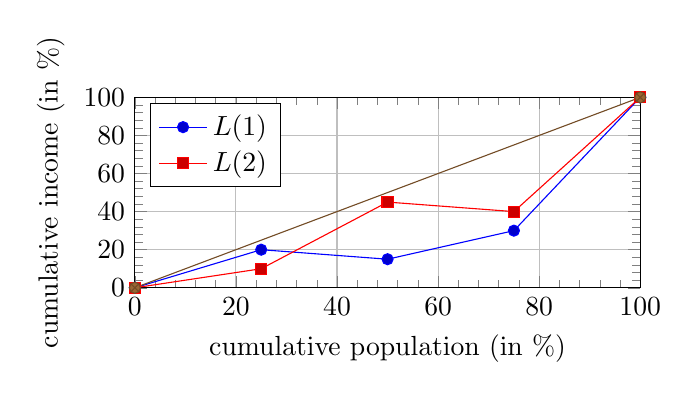
\begin{tikzpicture}
		\begin{axis}[
				xmin=0, xmax=100,
				ymin=0, ymax=100,
				minor tick num = 4,
				grid,
				ylabel = cumulative income (in \%),
				xlabel = cumulative population (in \%),
				legend style={legend pos=north west},
			]
			\addplot plot
			coordinates {(0,0) (25,20) (50,15) (75,30) (100,100)};
			\addplot plot
			coordinates {(0,0) (25,10) (50,45) (75,40) (100,100)};
			\addplot plot [thin]
			coordinates {(0,0) (100,100)};
			\legend{$L(1)$,$L(2)$}
		\end{axis}
	\end{tikzpicture}
\end{frame}

\begin{frame}{Gini Index (CART, IBM IntelligentMiner)}
	\begin{itemize}
		\item \textbf{If a dataset D contains examples from n classes, Gini index gini(D) is defined as:}
		      \begin{align}
			      \text{gini}(D) = 1-\sum_{j=1}^{n} p_j^2,
		      \end{align}
		      where $p_j$ is the relative frequency of class $j$ in $D$.
		\item \textbf{If a dataset $D$ is split on $A$ into two subsets $D_1$ and $D_2$, the Gini index $\text{gini}(D)$ is defined as}
		      \begin{align}
			      \text{gini}_A(D) = \frac{|D_1|}{|D|}\text{gini}(D_1)+\frac{|D_2|}{|D|}\text{gini}(D_2).
		      \end{align}
		\item \textbf{Reduction in impurity:}
		      \begin{align}
			      \Delta \text{gini}_A(D) = \text{gini}(D)-\text{gini}_A(D).
		      \end{align}
		\item \textbf{The attribute $A$ provides the smallest $\text{gini}_A(D)$ (or the largest reduction in impurity) \\ is chosen to split the node.}
		      \begin{itemize}
			      \item Need to enumerate all the possible splitting points for each attribute.
		      \end{itemize}
	\end{itemize}
\end{frame}


\begin{frame}{Computation of Gini Index (I)}
	\begin{itemize}
		\item \textbf{Example:}
		      \begin{itemize}
			      \item $D$ has $9$ tuples in $\text{buys\_computer} =$ "yes" and 5 in "no", thus
			            \begin{align}
				            \text{gini}(D) = 1 - \left( \frac{9}{14} \right)^2 - \left( \frac{5}{14} \right)^2 = 0.459.
			            \end{align}
		      \end{itemize}
		\item Suppose the attribute $\texttt{income}$ partitions $D$ \\ into $10$ in $D_1:\{\texttt{low,medium}\}$ and $4$ in $D_2: \{\texttt{high}\}$:
		      \begin{align}
			       & \text{gini}(D\vert_{D[\texttt{income}]="medium", "low"})                                                                                                                                   \\
			       & = \frac{10}{14} \text{gini}(D_1) + \frac{4}{14} \text{gini}(D_2)                                                                                                                           \\
			       & =\frac{10}{14} \left(1-\left( \frac{7}{10} \right)^2 - \left( \frac{3}{10} \right)^2 \right) + \frac{4}{14} \left( 1-\left( \frac{2}{4} \right)^2 - \left( \frac{2}{4} \right)^2 \right) = \\
			       & = 0.443 = \text{gini}(D\vert_{D[\texttt{income}]="high"}).
		      \end{align}
	\end{itemize}
\end{frame}

\begin{frame}{Computation of Gini Index (II)}
	\begin{itemize}
		\item \textbf{Example (cont.):}
		      \begin{itemize}
			      \item $\text{gini}(D\vert_{D[\texttt{income}]="low", "high"}) = 0.458$,\\
			            $\text{gini}(D\vert_{D[\texttt{income}]="medium", "high"}) = 0.450.$
			      \item Thus, split on the \{"low","medium"\} and \{"high"\}, since it has the lowest gini index.
		      \end{itemize}
		\item \textbf{All attributes are assumed continuous-valued.}
		\item \textbf{May need other tools, E.g., clustering, to get the possible split values.}
		\item \textbf{Can be modified for categorical attributes.}
	\end{itemize}
\end{frame}

\begin{frame}{Computation of Gini Index (III)}
	\begin{itemize}
		\item \textbf{The three measures, in general, return good results, but}
		      \begin{itemize}
			      \item \textbf{\color{airforceblue}Information gain:}
			            \begin{itemize}
				            \item Biased towards multi-valued attributes.
			            \end{itemize}
			      \item \textbf{\color{airforceblue}Gain ratio:}
			            \begin{itemize}
				            \item Tends to prefer unbalanced splits in which one partition is much smaller than the others.
			            \end{itemize}
			      \item \textbf{\color{airforceblue}Gini index:}
			            \begin{itemize}
				            \item Biased to multi-valued attributes.
				            \item Has difficulty when number of classes is large.
				            \item Tends to favor tests that result in equal-sized partitions and purity in both partitions.
			            \end{itemize}
		      \end{itemize}
	\end{itemize}
\end{frame}

\begin{frame}{Other Attribute-selection Measures}
	\begin{itemize}
		\item \textbf{CHAID:}
		      \begin{itemize}
			      \item A popular decision-tree algorithm, measure based on $\chi^2$ test for independence.
		      \end{itemize}
		\item \textbf{C-SEP:}
		      \begin{itemize}
			      \item Performs better than information gain and Gini index in certain cases.
		      \end{itemize}
		\item \textbf{G-statistic:}
		      \begin{itemize}
			      \item Has a close approximation to $\chi^2$ distribution.
		      \end{itemize}
		\item \textbf{MDL (Minimal Description Length) principle:}
		      \begin{itemize}
			      \item I.e. the simplest solution is preferred.
			      \item The best tree is the one that requires the fewest number of bits to both (1) encode the tree and (2) encode the exceptions to the tree.
		      \end{itemize}
		\item \textbf{Multivariate splits:}
		      \begin{itemize}
			      \item Partitioning based on multiple variable combinations.
			      \item CART: finds multivariate splits based on a linear combination of attributes.
		      \end{itemize}
		\item \textbf{Which attribute-selection measure is the best?}
		      \begin{itemize}
			      \item Most give good results, none is significantly superior to others.
		      \end{itemize}
	\end{itemize}
\end{frame}

\begin{frame}{Overfitting and Tree Pruning}
	\begin{itemize}
		\item \textbf{Overfitting: An induced tree may overfit the training data.}
		      \begin{itemize}
			      \item Too many branches, some may reflect anomalies due to noise or outliers.
			      \item Poor accuracy for unseen samples.
		      \end{itemize}
		\item \textbf{Two approaches to avoid overfitting:}
		      \begin{itemize}
			      \item \textbf{\color{airforceblue}Prepruning:}
			            \begin{itemize}
				            \item Halt tree construction early.\\
				                  Do not split a node, if this would result in the goodness measure falling below a threshold.
				            \item Difficult to choose an appropriate threshold.
			            \end{itemize}
			      \item \textbf{\color{airforceblue}Postpruning:}
			            \begin{itemize}
				            \item Remove branches from a "fully grown" tree.\\
				                  Get a sequence of progressively pruned trees.
				            \item Use a set of data different from the training data to decide which is the "best pruned tree."
			            \end{itemize}
		      \end{itemize}
	\end{itemize}
\end{frame}

\begin{frame}{Enhancements to Basic Decision-Tree Induction}
	\begin{itemize}
		\item \textbf{Allow for} \textbf{\color{airforceblue}continuous-valued attributes.}
		      \begin{itemize}
			      \item Dynamically define new discrete-valued attributes that partition the values of continuous-valued attributes into a discrete set of intervals.
		      \end{itemize}
		\item \textbf{Handle} \textbf{\color{airforceblue}missing attribute values.}
		      \begin{itemize}
			      \item Assign the most common value of the attribute.
			      \item Assign probability to each of the possible values.
		      \end{itemize}
		\item \textbf{\color{airforceblue}Attribute construction.}
		      \begin{itemize}
			      \item Create new attributes based on existing ones that are sparsely represented.
			      \item This reduces fragmentation, repetition, and replication.
		      \end{itemize}
	\end{itemize}
\end{frame}

\begin{frame}{Classification in Large Databases}
	\begin{itemize}
		\item \textbf{Classification -- a classical problem extensively \\ studied by statisticians and machine-learning researchers.}
		\item \textbf{Scalability:}
		      \begin{itemize}
			      \item Classifying datasets with millions of examples and \\ hundreds of attributes with reasonable speed.
		      \end{itemize}
		\item \textbf{Why is decision-tree induction popular?}
		      \begin{itemize}
			      \item Relatively fast learning speed (compared to other classification methods).
			      \item Convertible to simple and easy-to-understand classification rules.
			      \item Can use SQL queries for accessing databases.
			      \item Classification accuracy comparable with other methods.
		      \end{itemize}
		\item \textbf{RainForest (Gehrke, Ramakrishnan \& Ganti, VLDB'98).}
		      \begin{itemize}
			      \item Builds an AVC-list (attribute, value, class\_label).
		      \end{itemize}
	\end{itemize}
\end{frame}

\begin{frame}{Scalability Framework for RainForest}
	\begin{itemize}
		\item \textbf{Separates the scalability aspects from the criteria that determine the quality of the tree.}
		\item \textbf{Builds an} \textbf{\color{airforceblue}AVC-list:}.
		      \begin{itemize}
			      \item AVC (Attribute, Value, Class\_label).
		      \end{itemize}
		\item \textbf{\color{airforceblue}AVC-set} \textbf{(of an attribute X):}
		      \begin{itemize}
			      \item Projection of training dataset onto the attribute $X$ and class label where counts of individual class label are aggregated.
		      \end{itemize}
		\item \textbf{\color{airforceblue}AVC-group} \textbf{(of a node n):}
		      \begin{itemize}
			      \item Set of AVC-sets of all predictor attributes at the node $n$.
		      \end{itemize}
	\end{itemize}
\end{frame}

\begin{frame}{RainForest: Training Set and its AVC-sets}
	\begin{columns}
		\begin{column}{0.6\textwidth}
			\small
			\begin{tabular}{|l|l|c|c|c|}
	\hline
	\rowcolor{faugray!62}\textbf{age} & \textbf{income} & \textbf{student} & \textbf{credit\_rating} & \textbf{buys\_computer} \\\hline
	$\leq 30$                         & high            & no               & fair                    & {\color{faured}no}      \\\hline
	$\leq 30$                         & high            & no               & excellent               & {\color{faured}no}      \\\hline
	$31\ldots40$                      & high            & no               & fair                    & {\color{faugreen}yes}   \\\hline
	$>40$                             & medium          & no               & fair                    & {\color{faugreen}yes}   \\\hline
	$>40$                             & low             & yes              & fair                    & {\color{faugreen}yes}   \\\hline
	$>40$                             & low             & yes              & excellent               & {\color{faured}no}      \\\hline
	$31\ldots40$                      & low             & yes              & excellent               & {\color{faugreen}yes}   \\\hline
	$\leq 30$                         & medium          & no               & fair                    & {\color{faured}no}      \\\hline
	$\leq 30$                         & low             & yes              & fair                    & {\color{faugreen}yes}   \\\hline
	$>40$                             & medium          & yes              & fair                    & {\color{faugreen}yes}   \\\hline
	$\leq 30$                         & medium          & yes              & excellent               & {\color{faugreen}yes}   \\\hline
	$31\ldots40$                      & medium          & no               & excellent               & {\color{faugreen}yes}   \\\hline
	$31\ldots40$                      & high            & yes              & fair                    & {\color{faugreen}yes}   \\\hline
	$>40$                             & medium          & no               & excellent               & {\color{faured}no}      \\\hline
\end{tabular}

		\end{column}
		\begin{column}{0.3\textwidth}
			\vspace{-3cm}

			\centering
			AVC-set on age:\\
			\begin{tabular}{|c|c|c|}
				\hline
				age          & yes & no \\\hline
				$\leq 30$    & 2   & 3  \\\hline
				$31\ldots40$ & 4   & 0  \\\hline
				$>40$        & 3   & 2  \\\hline
			\end{tabular}\\[1cm]
			AVC-set on income:\\
			\begin{tabular}{|c|c|c|}
				\hline
				income & yes & no \\\hline
				high   & 2   & 2  \\\hline
				medium & 4   & 2  \\\hline
				low    & 3   & 1  \\\hline
			\end{tabular}
		\end{column}
	\end{columns}
\end{frame}

\begin{frame}{RainForest: Training Set and its AVC-sets (II)}
	\begin{columns}
		\begin{column}{0.6\textwidth}
			\small
			\begin{tabular}{|l|l|c|c|c|}
	\hline
	\rowcolor{faugray!62}\textbf{age} & \textbf{income} & \textbf{student} & \textbf{credit\_rating} & \textbf{buys\_computer} \\\hline
	$\leq 30$                         & high            & no               & fair                    & {\color{faured}no}      \\\hline
	$\leq 30$                         & high            & no               & excellent               & {\color{faured}no}      \\\hline
	$31\ldots40$                      & high            & no               & fair                    & {\color{faugreen}yes}   \\\hline
	$>40$                             & medium          & no               & fair                    & {\color{faugreen}yes}   \\\hline
	$>40$                             & low             & yes              & fair                    & {\color{faugreen}yes}   \\\hline
	$>40$                             & low             & yes              & excellent               & {\color{faured}no}      \\\hline
	$31\ldots40$                      & low             & yes              & excellent               & {\color{faugreen}yes}   \\\hline
	$\leq 30$                         & medium          & no               & fair                    & {\color{faured}no}      \\\hline
	$\leq 30$                         & low             & yes              & fair                    & {\color{faugreen}yes}   \\\hline
	$>40$                             & medium          & yes              & fair                    & {\color{faugreen}yes}   \\\hline
	$\leq 30$                         & medium          & yes              & excellent               & {\color{faugreen}yes}   \\\hline
	$31\ldots40$                      & medium          & no               & excellent               & {\color{faugreen}yes}   \\\hline
	$31\ldots40$                      & high            & yes              & fair                    & {\color{faugreen}yes}   \\\hline
	$>40$                             & medium          & no               & excellent               & {\color{faured}no}      \\\hline
\end{tabular}

		\end{column}
		\begin{column}{0.3\textwidth}
			\vspace{-3cm}

			\centering
			AVC-set on student:\\
			\begin{tabular}{|c|c|c|}
				\hline
				student & yes & no \\\hline
				yes     & 6   & 1  \\\hline
				no      & 3   & 4  \\\hline
			\end{tabular}\\[1cm]
			AVC-set on credit\_rating:\\
			\begin{tabular}{|c|c|c|}
				\hline
				credit\_rating & yes & no \\\hline
				fair           & 6   & 2  \\\hline
				excellent      & 3   & 3  \\\hline
			\end{tabular}
		\end{column}
	\end{columns}
\end{frame}

\begin{frame}{BOAT (Bootstrapped Optimistic Algorithm for Tree Construction)}
	\begin{itemize}
		\item \textbf{Use a statistical technique called bootstrapping to create several smaller samples (subsets), each fitting in memory.}
		      \begin{itemize}
			      \item See on the subsequent slides.
		      \end{itemize}
		\item \textbf{Each subset is used to create a tree, resulting in several trees.}
		\item \textbf{These trees are examined and used to construct a new tree T'.}
		      \begin{itemize}
			      \item It turns out that T' is very close to the tree that would be generated \\
			            using the whole data set together.
		      \end{itemize}
		\item \textbf{Advantages:}
		      \begin{itemize}
			      \item Requires only two scans of DB.
			      \item An incremental algorithm:
			            \begin{itemize}
				            \item Take insertions and deletions of training data and update the decision tree.
			            \end{itemize}
		      \end{itemize}
	\end{itemize}
\end{frame}

\begin{frame}{Presentation of Classification Results}
	\centering
	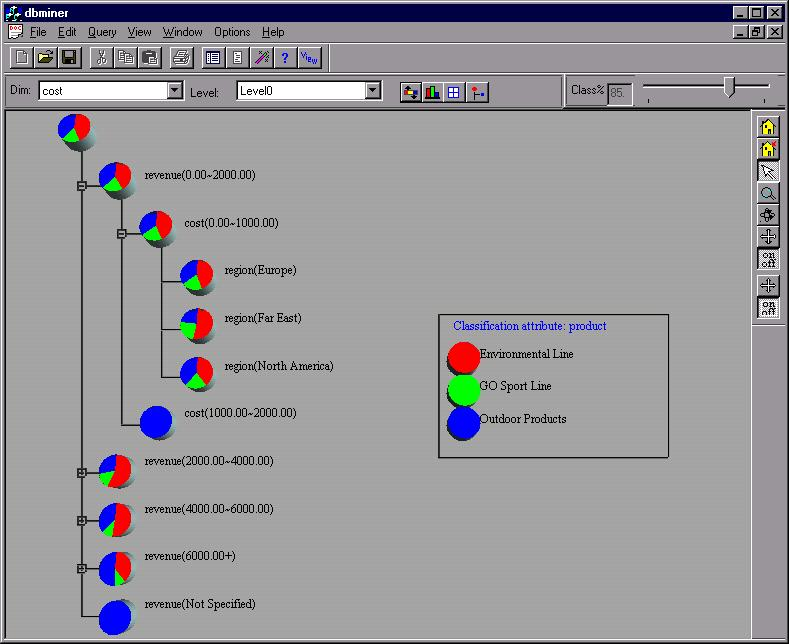
\includegraphics[height=0.8\textheight]{img/classification1.jpeg}
\end{frame}

\begin{frame}{Visualization of a Decision Tree in SGI/MineSet 3.0}
	\centering
	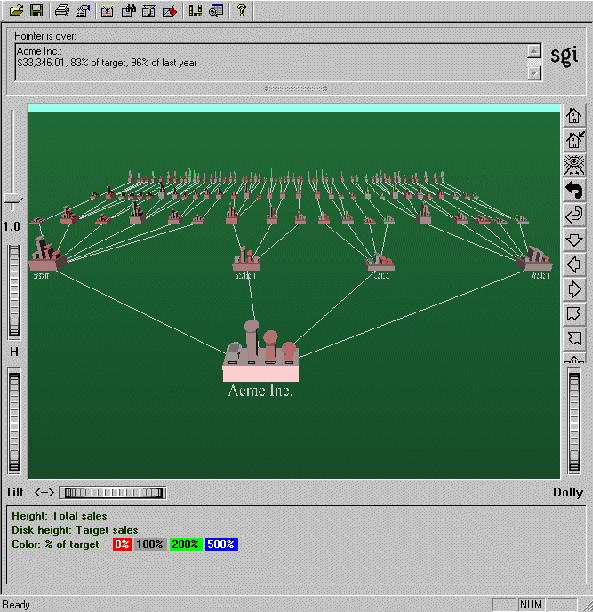
\includegraphics[height=0.8\textheight]{img/classification2.jpeg}
\end{frame}

\begin{frame}{Interactive Visual Mining by Perception-based Classification (PBC)}
	\centering
	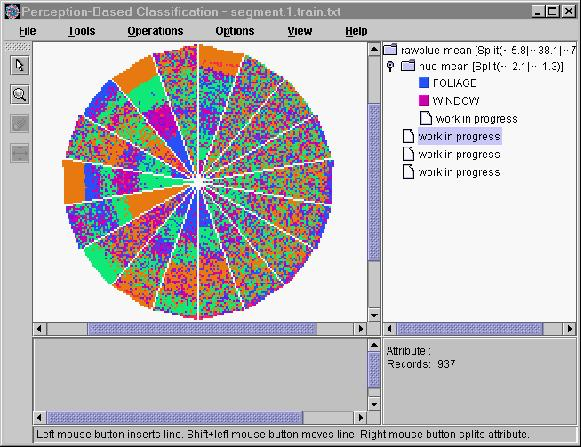
\includegraphics[height=0.8\textheight]{img/classification3.jpeg}
\end{frame}

\section{Rule-Based Classification}

\begin{frame}{Using \uppercase{if-then} Rules for Classification}
	\begin{itemize}
		\item \textbf{Represent the knowledge in the form of {\color{airforceblue}IF-THEN rules}.}
		      \begin{itemize}
			      \item E.g., if \texttt{age} $\leq 30$ AND \texttt{student} = "yes" THEN buys\_computer = "yes".
			      \item Readable.
		      \end{itemize}
		\item \textbf{Rule {\color{airforceblue}antecedent/precondition} vs. rule {\color{airforceblue}consequent}}.
		\item \textbf{Assessment of a rule R: coverage and accuracy.}
		      \begin{itemize}
			      \item $n_{\text{covers}} = \#$ of tuples covered by $R$ (antecedent if true).
			      \item $n_{\text{correct}} = \#$ of tuples correctly classified by $R$.
			      \item $\text{coverage}(R) = \frac{n_{\text{covers}}}{|D|}$ with $D$ training data set.
			      \item $\text{accuracy}(R) = \frac{n_{\text{correct}}}{n_{\text{covers}}}$.
		      \end{itemize}
	\end{itemize}
\end{frame}

\begin{frame}[c]{Potential Problems of Rule-Based Classification}
	\centering
	\huge
	\begin{enumerate}
		\item More than one rule is triggered.
		\item No rule is triggered.
	\end{enumerate}
\end{frame}

\begin{frame}{Potential Problems of Rule-based Classification: Solutions}
	\begin{enumerate}
		\item \textbf{More than one rule is triggered: {\color{airforceblue}conflict resolution}.}
		      \begin{itemize}
			      \item \textbf{\color{airforceblue}Size ordering:}
			            \begin{itemize}
				            \item Assign the highest priority to the triggered rule that has the "toughest" requirement \\ (i.e., rule with most used attribute in condition).
			            \end{itemize}
			      \item \textbf{\color{airforceblue}Class-based ordering:}
			            \begin{itemize}
				            \item Decreasing order of prevalence or misclassification cost per class.
				            \item No order of rules within class $\rightarrow$ disjunction (logical \texttt{OR}) between rules.
			            \end{itemize}
			      \item \textbf{\color{airforceblue}Rule-based ordering} (decision list):
			            \begin{itemize}
				            \item Rules are organized into one long priority list,\\
				                  according to some measure of rule quality, or by experts.
				            \item Rules \underline{must} be applied in this particular order to avoid conflict.
			            \end{itemize}
		      \end{itemize}
		\item \textbf{No rule is triggered.}
		      \begin{itemize}
			      \item Use a fallback/default rule.
			      \item Always evaluated as the last rule, if and only if other rules are not covered by some tuple, i. e. no rules have been triggered.
		      \end{itemize}
	\end{enumerate}
\end{frame}

\begin{frame}{Rule Extraction from a Decision Tree}
	\begin{itemize}
		\item \textbf{Rules are {\color{airforceblue}easier to understand} than large trees.}
		\item \textbf{Rule can be created for {\color{airforceblue}each path from the root to a leaf.}}
		      \begin{itemize}
			      \item The leaf holds the class prediction.
		      \end{itemize}
		\item \textbf{Each attribute-value pair along the path forms a conjunction:}
	\end{itemize}
	\vspace*{1em}
	\begin{columns}
		\begin{column}{0.55\textwidth}
			\textbf{Example:}
			\begin{enumerate}
				\item IF \texttt{age} $\leq$ 30 AND \texttt{student} = "no" \\
				      THEN \texttt{buys\_computer} = "no".
				\item IF \texttt{age} $\leq$ 30 AND \texttt{student} = "yes" \\
				      THEN \texttt{buys\_computer} = "yes".
				\item IF \texttt{age}== $31\ldots40$ THEN \texttt{buys\_computer} = "yes".
				\item \dots
			\end{enumerate}
		\end{column}
		\begin{column}{0.45\textwidth}
			\vspace*{-1em}
			\begin{figure}[h]
				\centering
				\begin{tikzpicture}
	\node[rounded corners=.25em,draw, fill=faugray!62] at (0,0) (a) {age?};
	\node[rounded corners=.25em,draw] at (-1.5,-0.7) (b) {<=30};
	\node[rounded corners=.25em,draw] at (0,-0.7) (c) {$31\ldots40$};
	\node[rounded corners=.25em,draw] at (1.5,-0.7) (d) {$>40$};
	\node[rounded corners=.25em,draw, fill=faugray!62] at (-1.5,-1.4) (e) {student?};
	\node[rounded corners=.25em,draw] at (-2,-2.1) (eno1) {no};
	\node[rounded corners=.25em,draw] at (-1,-2.1) (eyes1) {yes};
	\node[text=faured] at (-2,-2.8) (eno2) {no};
	\node[text=faugreen] at (-1,-2.8) (eyes2) {yes};
	\node[rounded corners=.25em,draw,fill=faugray!62] at (1.5,-1.4) (g) {credit rating?};
	\node[rounded corners=.25em,draw] at (2.2,-2.1) (gf) {fair};
	\node[rounded corners=.25em,draw] at (1,-2.1) (gex) {excellent};
	\node[text=faured] at (1,-2.8) (gno) {no};
	\node[text=faugreen] at (2.2,-2.8) (gyes) {yes};
	\node[text=faugreen] at (0,-2.8) (f) {yes};

	\draw (a)--(b);
	\draw (a)--(c);
	\draw (a)--(d);
	\draw (b)--(e);
	\draw (c)--(f);
	\draw (d)--(g);
	\draw (e)--(eno1);
	\draw (e)--(eyes1);
	\draw (eno1)--(eno2);
	\draw (eyes1)--(eyes2);
	\draw (g)--(gex);
	\draw (g)--(gf);
	\draw (gex)--(gno);
	\draw (gf)--(gyes);
\end{tikzpicture}

			\end{figure}
		\end{column}
	\end{columns}
\end{frame}

\begin{frame}{Rule Induction: Sequential Covering Method}
	\begin{itemize}
		\item \textbf{Sequential covering algorithm:}
		      \begin{itemize}
			      \item Extracts rules directly from training data.
		      \end{itemize}
		\item \textbf{Typical sequential covering algorithms:}
		      \begin{itemize}
			      \item FOIL, AQ, CN2, RIPPER.
		      \end{itemize}
		\item \textbf{Rules are learned {\color{airforceblue}sequentially}.}
		      \begin{itemize}
			      \item Each rule for a given class $C_i$ will cover many tuples of $C_i$, but none (or few) of the tuples of other classes.
		      \end{itemize}
		\item \textbf{Algorithm sketch:}
		      \begin{itemize}
			      \item Rules are learned one at a time.
			      \item Each time a rule is learned, the tuples covered by the rule are removed.
			      \item The process repeats on the remaining tuples unless termination condition, e.g., when no more training examples left or when the quality of a rule returned is below a user-specified threshold.
		      \end{itemize}
		\item \textbf{Compare with decision-tree induction:}
		      \begin{itemize}
			      \item That was learning a set of rules simultaneously.
		      \end{itemize}
	\end{itemize}
\end{frame}

\begin{frame}{Sequential Covering Algorithm (I)}
	% REVIEW: This header is a bit confusing after concrete Sequential Covering Algortihms are presented on the previous slide. One wonders which of the algorithms is being outlined here. Since "FOIL_Gain" is mentioned on the next slide, I assume that the algorithm outlined here is supposed to be FOIL. Accordingly, I would then also mention this in the three headers.
	\begin{itemize}
		\item \textbf{While (enough target tuples left):}
		      \begin{itemize}
			      \item generate a rule;
			      \item remove positive target tuples satisfying this rule;
		      \end{itemize}
		      \centering
		      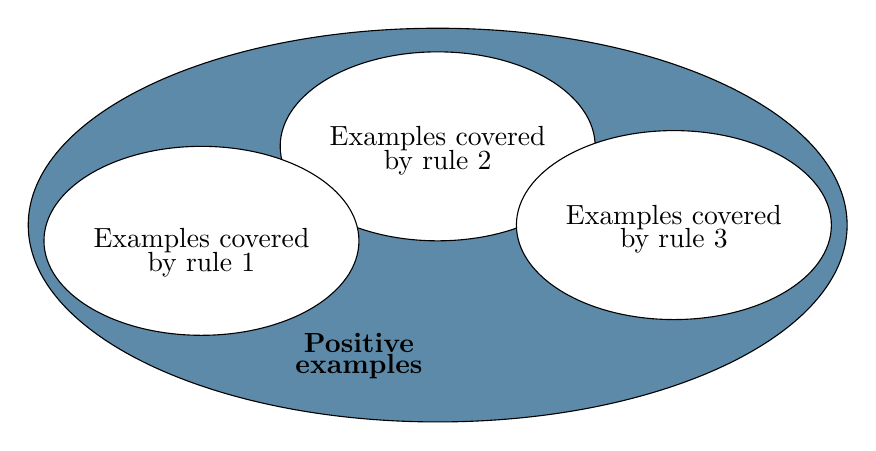
\begin{tikzpicture}
			      \draw[fill=airforceblue] (0,0) ellipse (5.2 and 2.5) (0,0) node [text=black] {};
			      \draw[fill=white] (0,1) ellipse (2 and 1.2) (0,0) node [text=black] {};
			      \draw[fill=white] (-3,-0.2) ellipse (2 and 1.2) (0,0) node [text=black] {};
			      \draw[fill=white] (3,0) ellipse (2 and 1.2) (0,0) node [text=black] {};
			      \node at (0,1.1) (a1) {Examples covered};
			      \node at (0,0.8) (a2) {by rule 2};
			      \node at (3,0.1) (b1) {Examples covered};
			      \node at (3,-0.2) (b2) {by rule 3};
			      \node at (-3,-0.2) (c1) {Examples covered};
			      \node at (-3,-0.5) (c2) {by rule 1};
			      \node at (-1,-1.5) (d1) {\textbf{Positive}};
			      \node at (-1,-1.8) (d2) {\textbf{examples}};
		      \end{tikzpicture}
	\end{itemize}
\end{frame}

\begin{frame}{Sequential Covering Algorithm (II)}
	\begin{itemize}
		\item \textbf{To generate a rule:}
		      \begin{itemize}
			      \item \textbf{while}(true:)
			            \begin{itemize}
				            \item find the best predicate $p$ (attribute = value);
				            \item \textbf{if} \texttt{FOIL\_Gain}(p) > threshold
				            \item \textbf{then} add $p$ to current rule;
				            \item \textbf{else} break;
			            \end{itemize}
		      \end{itemize}
	\end{itemize}
	\centering
	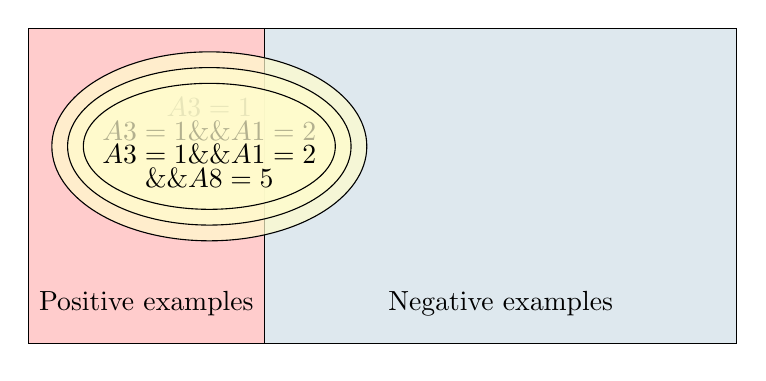
\begin{tikzpicture}
		\draw[fill=red!20] (-3,0) rectangle (1,4) (0,0) node [text=black] {};
		\draw[fill=airforceblue!20] (6,0) rectangle (0,4) (0,0) node [text=black] {};
		\node at (3,0.5) (a1) {Negative examples};
		\node at (-1.5,0.5) (a1) {Positive examples};
		\uncover<2->{
			\draw[fill=yellow!20,fill opacity=0.7] (-0.7,2.5) ellipse (2 and 1.2) (0,0) node [text=black] {};
			\node at (-0.7,3) {$A3=1$};
		}
		\uncover<3->{
			\draw[fill=yellow!20,fill opacity=0.7] (-0.7,2.5) ellipse (1.8 and 1) (0,0) node [text=black] {};
			\node at (-0.7,2.7) {$A3=1 \&\& A1=2$};
		}
		\uncover<4->{
			\draw[fill=yellow!20,fill opacity=0.7] (-0.7,2.5) ellipse (1.6 and 0.8) (0,0) node [text=black] {};
			\node at (-0.7,2.4) {$A3=1 \&\& A1=2$};
			\node at (-0.7,2.1) {$\&\& A8=5$};
		}
	\end{tikzpicture}
\end{frame}

% TODO: Review again and cosmetics
\begin{frame}{Sequential Covering Algorithm (III)}
	\begin{itemize}
		\item \textbf{Start with the most general rule possible:}
		      \begin{itemize}
			      \item Condition = empty.
		      \end{itemize}
		\item \textbf{Add new attributes by adopting a greedy depth-first strategy.}
		      \begin{itemize}
			      \item Pick the one that improves the rule quality most.
			      \item Current rule $R$: IF condition THEN class = c.
			      \item New rule $R'$: IF condition' THEN class = c,
			      \item $pos/neg$ are $\#$ of positive/negative tuples covered by $R$.
		      \end{itemize}
		\item \textbf{Rule-quality measures.}
		      \begin{itemize}
			      \item Must consider both coverage and accuracy.
			      \item \texttt{FOIL\_Gain} (from \texttt{FOIL} - First-Order Inductive Learner):
			            \begin{align*}
				            \text{FOIL\_Gain} = \text{pos}' \left( \log_2 \frac{\text{pos}'}{\text{pos}' + \text{neg}'} - \log_2 \frac{\text{pos}}{\text{pos}+\text{neg}} \right).
			            \end{align*}
			      \item Favors rules that have high accuracy and cover many positive tuples.
		      \end{itemize}
	\end{itemize}
\end{frame}

\begin{frame}{Rule Pruning}
	\begin{itemize}
		\item \textbf{Danger of {\color{airforceblue}overfitting}.}
		\item \textbf{Removing a conjunct (attribute test),}
		      \begin{itemize}
			      \item if pruned version of rule has greater quality,\\
			            assessed on an independent set of test tuples (called "pruning set").
		      \end{itemize}
		\item \textbf{FOIL uses:}
		      \begin{align*}
			      \text{FOIL\_Prune}(R) = \frac{\text{pos}-\text{neg}}{\text{pos}+\text{neg}}.
		      \end{align*}
		\item If $\text{FOIL\_Prune}$ is higher for the pruned version of $R$, prune $R$.
	\end{itemize}
\end{frame}

\section{Bayes Classification Methods}

\begin{frame}{Bayesian Classification: Why?}
	\begin{itemize}
		\item \textbf{A statistical classifier:}
		      \begin{itemize}
			      \item Performs probabilistic prediction, i.e. predicts class-membership probabilities.
		      \end{itemize}
		\item \textbf{Foundation:} \textbf{\color{airforceblue}Bayes' Theorem.}
		\item \textbf{Performance:}
		      \begin{itemize}
			      \item A simple Bayesian classifier (naïve Bayesian classifier) has performance comparable with decision tree and selected neural-network classifiers.
		      \end{itemize}
		\item \textbf{Incremental:}
		      \begin{itemize}
			      \item Each training example can incrementally increase/decrease the probability that a hypothesis is correct -- prior knowledge can be combined with observed data.
		      \end{itemize}
		\item \textbf{Standard:}
		      \begin{itemize}
			      \item Even when Bayesian methods are computationally intractable, they can provide a standard of optimal decision making against which other methods can be measured.
		      \end{itemize}
	\end{itemize}
\end{frame}

\begin{frame}{Bayes' Theorem: Basics}
	\begin{itemize}
		\item \textbf{Let $X$ be a data sample ("evidence").}
		      \begin{itemize}
			      \item The class label shall be unknown.
		      \end{itemize}
		\item \textbf{Let $C_i$ be the hypothesis that $X$ belongs to class $i$.}
		\item \textbf{Classification is to determine $P(C_i|X)$:}
		      \begin{itemize}
			      \item \textbf{\color{airforceblue}Posteriori probability:} the probability that the hypothesis \\ holds given the observed data sample $X$.
		      \end{itemize}
		\item $P(C_i)$:
		      \begin{itemize}
			      \item \textbf{\color{airforceblue}Prior probability:} the initial probability.
			      \item E.g., $X$ will buy computer, regardless of age, income, $\ldots$
		      \end{itemize}
		\item $P(X)$:
		      \begin{itemize}
			      \item Probability that sample data is observed.
		      \end{itemize}
		\item $P(X|C_j)$:
		      \begin{itemize}
			      \item \textbf{\color{airforceblue}Likelihood:} the probability of observing the sample $X$ given that the hypothesis holds.
			      \item E.g., given that $X$ buys computer, the probability that $X$ is $31\ldots40$, medium income.
		      \end{itemize}
	\end{itemize}
\end{frame}

\begin{frame}{Bayes' Theorem (II)}
	\begin{itemize}
		\item \textbf{Given training data $X$, the posteriori probability $P(C_i|X)$\\
			      of a hypothesis $C_i$ follows from the Bayes' Theorem:}
		      \begin{align}
			      P(C_i|X) = \frac{P(X|C_i)P(C_i)}{P(X)}.
		      \end{align}
		\item \textbf{Predicts that $X$ belongs to $C_i$ if the probability $P(C_i|X)$\\
			      is {\color{airforceblue}the highest} among all the $P(C_k|X)$ for all $k$ classes.}
		\item \textbf{Practical difficulty:}
		      \begin{itemize}
			      \item Requires initial knowledge of many probabilities.
			      \item Significant computational cost.
		      \end{itemize}
	\end{itemize}
\end{frame}

\begin{frame}{Towards Naïve Bayesian Classifier}
	\begin{itemize}
		\item \textbf{Let $D$ be a training set of tuples and their associated class labels.}
		      \begin{itemize}
			      \item Each tuple is represented by an $n$-dimensional attribute $X = (x_1,x_2,\ldots,x_n)$.
		      \end{itemize}
		\item \textbf{Supose there are $m$ classes $C_1,C_2, \ldots, C_m$.}
		\item \textbf{Classification is to derive the {\color{airforceblue}maximum posteriori probability}.}
		      \begin{itemize}
			      \item i.e. the maximal $P(C_i|X)$.
		      \end{itemize}
		\item \textbf{This can be derived from Bayes' Theorem:}
		      \begin{align}
			      P(C_i|X) = \frac{P(X|C_i)P(C_i)}{P(X)}.
		      \end{align}
		\item \textbf{Since $P(X)$ is constant for all classes, we must maximize only:}
		      \begin{align}
			      P(X|C_i)P(C_i).
		      \end{align}
	\end{itemize}
\end{frame}

\begin{frame}{Derivation of Naïve Bayes Classifier}
	\begin{itemize}
		\item \textbf{A simplifying assumption: attributes are {\color{airforceblue}conditionally independent}.}
		      \begin{itemize}
			      \item I.e. no dependence relation between attributes (which is "naïve").
			            \begin{align*}
				            \resizebox{7cm}{!}{%
					            $P(X|C_i) = \prod_{k=1}^{n} P(x_k|C_i) = P(x_1|C_i)P(x_2|C_i)\cdots P(x_n|C_i).$}
			            \end{align*}
			      \item This greatly reduces the computation cost:\\
			            Only count the class distribution.
			      \item If $A_k$ is categorical,
			            \begin{itemize}
				            \item $P(x_k|C_i)$is the number of tuples in $C_i$ having value $x_k$ for $A_k$ \\
				                  divided by $|C_{i,D}|$ (the number of tuples of $C_i$ in $D$).
			            \end{itemize}
			      \item If $A_k$ is continuous-valued,
			            \begin{itemize}
				            \item $P(x_k|C_i)$ is usually computed based on Gaussian distribution with a mean $\mu$ and standard deviation $\sigma$:
				                  \begin{align*}
					                  \resizebox{4cm}{!}{%
					                  $G(x,\mu,\sigma) = \frac{1}{\sqrt{2\pi}\sigma}e^{\frac{(x-\mu)^2}{2\sigma^2}},$}
				                  \end{align*}
				            \item and $P(x_k|C_i) = G(x_k,\mu_{C_i},\sigma_{C_i})$.
			            \end{itemize}
		      \end{itemize}
	\end{itemize}
\end{frame}

\begin{frame}{Naïve Bayesian Cellcolormake Dataset}
	\begin{columns}
		\begin{column}{0.4\textwidth}
			\vspace{-2cm}
			\begin{itemize}
				\item \textbf{Classes:}
				      \begin{itemize}
					      \item $C_1$: \texttt{buys\_computer} = "yes".
					      \item $C_2$: \texttt{buys\_computer} = "no".
				      \end{itemize}
				\item \textbf{Data sample:}
				      \begin{itemize}
					      \item $X = (\texttt{age} \leq 30,$ \\
					            $\texttt{income} = "medium",$ \\
					            $\texttt{student} = "yes",$\\
					            $\texttt{credit\_rating} = "fair")$.
				      \end{itemize}
			\end{itemize}
		\end{column}
		\begin{column}{0.6\textwidth}
			\resizebox{\columnwidth}{!}{%
				\begin{tabular}{|l|l|c|c|c|}
	\hline
	\rowcolor{faugray!62}\textbf{age} & \textbf{income} & \textbf{student} & \textbf{credit\_rating} & \textbf{buys\_computer} \\\hline
	$\leq 30$                         & high            & no               & fair                    & {\color{faured}no}      \\\hline
	$\leq 30$                         & high            & no               & excellent               & {\color{faured}no}      \\\hline
	$31\ldots40$                      & high            & no               & fair                    & {\color{faugreen}yes}   \\\hline
	$>40$                             & medium          & no               & fair                    & {\color{faugreen}yes}   \\\hline
	$>40$                             & low             & yes              & fair                    & {\color{faugreen}yes}   \\\hline
	$>40$                             & low             & yes              & excellent               & {\color{faured}no}      \\\hline
	$31\ldots40$                      & low             & yes              & excellent               & {\color{faugreen}yes}   \\\hline
	$\leq 30$                         & medium          & no               & fair                    & {\color{faured}no}      \\\hline
	$\leq 30$                         & low             & yes              & fair                    & {\color{faugreen}yes}   \\\hline
	$>40$                             & medium          & yes              & fair                    & {\color{faugreen}yes}   \\\hline
	$\leq 30$                         & medium          & yes              & excellent               & {\color{faugreen}yes}   \\\hline
	$31\ldots40$                      & medium          & no               & excellent               & {\color{faugreen}yes}   \\\hline
	$31\ldots40$                      & high            & yes              & fair                    & {\color{faugreen}yes}   \\\hline
	$>40$                             & medium          & no               & excellent               & {\color{faured}no}      \\\hline
\end{tabular}

			}
		\end{column}
	\end{columns}
\end{frame}

\begin{frame}{Naïve Bayesian Classifier: An Example}
	\begin{itemize}
		\item $P(C_i)$:
		      \begin{itemize}
			      \item $P(\texttt{buys\_computer} = "yes") = \frac{9}{14} = 0.643$.
			      \item $P(\texttt{buys\_computer} = "no") = \frac{5}{14} = 0.357$.
		      \end{itemize}
		\item $X = (\texttt{age} \leq 30 , \texttt{income} = "medium", \texttt{student} = "yes", \texttt{credit\_rating} = "fair")$.
		\item \textbf{Compute $P(X|C_i)$ for each class:}
		      \begin{itemize}
			      \item $P(\texttt{age} \leq 30 | \texttt{buys\_computer} = "yes") = \frac{2}{9} = 0.222$.
			      \item $P(\texttt{age} \leq 30 | \texttt{buys\_computer} = "no") = \frac{3}{5} = 0.6$.
			      \item $P(\texttt{income} = "medium" | \texttt{buys\_computer} = "yes") = \frac{4}{9} = 0.444$.
			      \item $P(\texttt{income} = "medium" | \texttt{buys\_computer} = "no") = \frac{2}{5} = 0.4$.
			      \item $P(\texttt{student} = "yes" | \texttt{buys\_computer} = "yes") = \frac{6}{9} = 0.667$.
			      \item $P(\texttt{student} = "yes" | \texttt{buys\_computer} = "no") = \frac{1}{5} = 0.2$.
			      \item $P(\texttt{credit\_rating} = "fair" | \texttt{buys\_computer} = "yes") = \frac{6}{9} = 0.667$.
			      \item $P(\texttt{credit\_rating} = "fair" | \texttt{buys\_computer} = "no") = \frac{2}{5} = 0.4$.
		      \end{itemize}
	\end{itemize}
\end{frame}

\begin{frame}{Naïve Bayesian Classifier: An Example (II)}
	\begin{itemize}
		\item $P(C_i)$:
		      \begin{itemize}
			      \item $P(X | \texttt{buys\_computer} = "yes") = 0.222 \cdot 0.444 \cdot 0.667 \cdot 0.667 = 0.044$.
			      \item $P(X | \texttt{buys\_computer} = "no") = 0.6 \cdot 0.4 \cdot 0.2 \cdot 0.4 = 0.019$.
		      \end{itemize}
		\item $P(X | C_i) \cdot P(C_i)$:
		      \begin{itemize}
			      \item $P(X | \texttt{buys\_computer} = "yes") \cdot  P(\texttt{buys\_computer} = "yes") = 0.028$.
			      \item $P(X | \texttt{buys\_computer} = "no") \cdot  P(\texttt{buys\_computer} = "no") = 0.007$.
		      \end{itemize}
		\item \textbf{Therefore, $X$ belongs to class $C_1$ (\texttt{buys\_computer} = "yes")}.
	\end{itemize}
\end{frame}

\begin{frame}{Avoiding the Zero-probability Problem}
	\begin{itemize}
		\item \textbf{Naïve Bayesian prediction requires each conditional probability to be non-zero.}
		      \begin{itemize}
			      \item Otherwise, the predicted probability will be zero.
			            \begin{align}
				            \resizebox{4cm}{!}{
					            $P(X|C_i) = \prod_{k=1}^{n} P(x_k|C_i).$}
			            \end{align}
		      \end{itemize}
		\item \textbf{Example:}
		      \begin{itemize}
			      \item Suppose a dataset with $1000$ tuples, \texttt{income} = "low" $(0)$, \texttt{income} = "medium" $(990)$, and \texttt{income} = "high" $(10)$.
		      \end{itemize}
		\item \textbf{Use {\color{airforceblue}Laplacian correction} (or Laplacian estimator):}
		      \begin{itemize}
			      \item Add $1$ to each case:
			            \begin{itemize}
				            \item $P(\texttt{income} = "low") = \frac{1}{1003}$.
				            \item $P(\texttt{income} = "medium") = \frac{991}{1003}$.
				            \item $P(\texttt{income} = "high") = \frac{11}{1003}$.
			            \end{itemize}
			      \item The "corrected" probability estimates are close to their "uncorrected" counterparts.
		      \end{itemize}
	\end{itemize}
\end{frame}

\begin{frame}{Naïve Bayesian Classifier: Comments}
	\textbf{Advantages}
	\begin{itemize}
		\item Easy to implement.
		\item Good results obtained in most of the cases.
	\end{itemize}

	\textbf{Disadvantages}
	\begin{itemize}
		\item Assumption: class conditional independence, therefore loss of accuracy.
		\item Practically, \textbf{dependencies} exist among variables.
		      \begin{itemize}
			      \item E.g., hospital patients:
			            \begin{itemize}
				            \item Profile: age, family history, etc.
				            \item Symptoms: fever, cough, etc.
				            \item Disease: lung cancer, diabetes, etc.
			            \end{itemize}
			      \item Cannot be modeled by naïve Bayesian classifier.
		      \end{itemize}
	\end{itemize}

	\textbf{How to deal with these dependencies?} $\rightarrow$ Bayesian belief networks (see textbook).
\end{frame}

\section{Model Evaluation and Selection}\label{section:evaluation}

\begin{frame}{Model Evaluation and Selection}
	\begin{itemize}
		\item \textbf{Evaluation metrics:}
		      \begin{itemize}
			      \item How can we measure accuracy?
			      \item Other metrics to consider?
		      \end{itemize}
		\item \textbf{Use {\color{airforceblue}test} set of class-labeled tuples instead of training set when assessing accuracy.}
		\item \textbf{Methods for estimating a classifier's accuracy:}
		      \begin{itemize}
			      \item Holdout method, random subsampling.
			      \item Cross-validation.
			      \item Bootstrap.
		      \end{itemize}
		\item \textbf{Comparing classifiers:}
		      \begin{itemize}
			      \item Confidence intervals.
			      \item Cost-benefit analysis and ROC curves.
		      \end{itemize}
	\end{itemize}
\end{frame}

\begin{frame}{Confusion Matrix and Evaluation Metrics}
	Given $M$ classes, an entry $C^{(m)}_{ij}$ in an $M \times M$ confusion matrix
	indicates the number of tuples in class $i$ that were labeled by the
	classifier as class $j$.
	\begin{columns}[T]
	\begin{column}[T]{0.45\textwidth}
		\begin{tabular}{c|c|p{1cm}|p{1cm}|c|}

			\multicolumn{2}{c|}{\multirow{2}{*}{}} & \multicolumn{2}{c|}{Predicted Class} &                                           \\\cline{3-4}
			\multicolumn{2}{c|}{}                  & $C_1$                                & $\neg C_1$  & Total                       \\\hline
			\multirow{2}{*}{True Class}            & $C_1$                                & \textbf{TP} & \textbf{FN}    & \textbf{P} \\\cline{2-4}
			                                       & $\neg C_1$                           & \textbf{FP} & \textbf{TN}    & \textbf{N} \\\hline
			\multicolumn{2}{r|}{Total}             & \textbf{P'}                          & \textbf{N'} & \textbf{P + N}
		\end{tabular}

	\end{column}

	\begin{column}[T]{0.5\textwidth}
		\footnotesize
		\begin{itemize}
			\item \textbf{True Positives} = correctly classified tuples.
			\item \textbf{True Negatives} = correctly classified tuples.
			\item \textbf{False Positives} = negative tuples incorrectly classified as positive.
			\item \textbf{False Negatives} = positive tuples incorrectly classified as negative.
		\end{itemize}
	\end{column}
\end{columns}


	\textbf{Accuracy:}
	\vspace*{-1em}
	\begin{columns}
		\begin{column}{0.55\textwidth}
			\begin{itemize}
				\item Percentage of correctly classified tuples.
				\item Also known as the (overall) recognition rate.
				\item Most effective with a \textit{balanced dataset}.
				\item Inverse: \textbf{Error rate} as the misclassification rate.
			\end{itemize}
		\end{column}
		\begin{column}{0.4\textwidth}
			\vspace*{-1.2em}
			\begin{align*}
				\text{Accuracy}   & = \frac{\text{TP} + \text{TN}}{\text{P} +  \text{N}} \\
				\text{Error Rate} & = 1 - \text{Accuracy}                                \\
				                  & = \frac{\text{FP} + \text{FN}}{\text{P} + \text{N}}
			\end{align*}
		\end{column}
	\end{columns}
\end{frame}

\begin{frame}{Confusion Matrix and Evaluation Metrics (II)}
	\begin{columns}[T]
	\begin{column}[T]{0.45\textwidth}
		\begin{tabular}{c|c|p{1cm}|p{1cm}|c|}

			\multicolumn{2}{c|}{\multirow{2}{*}{}} & \multicolumn{2}{c|}{Predicted Class} &                                           \\\cline{3-4}
			\multicolumn{2}{c|}{}                  & $C_1$                                & $\neg C_1$  & Total                       \\\hline
			\multirow{2}{*}{True Class}            & $C_1$                                & \textbf{TP} & \textbf{FN}    & \textbf{P} \\\cline{2-4}
			                                       & $\neg C_1$                           & \textbf{FP} & \textbf{TN}    & \textbf{N} \\\hline
			\multicolumn{2}{r|}{Total}             & \textbf{P'}                          & \textbf{N'} & \textbf{P + N}
		\end{tabular}

	\end{column}

	\begin{column}[T]{0.5\textwidth}
		\footnotesize
		\begin{itemize}
			\item \textbf{True Positives} = correctly classified tuples.
			\item \textbf{True Negatives} = correctly classified tuples.
			\item \textbf{False Positives} = negative tuples incorrectly classified as positive.
			\item \textbf{False Negatives} = positive tuples incorrectly classified as negative.
		\end{itemize}
	\end{column}
\end{columns}

	\begin{columns}
		\begin{column}{0.4\textwidth}
			\begin{itemize}
				\item \textbf{Sensitivity} = True positive rate.
				\item \textbf{Specificity} = True negative rate.
				\item \textbf{Precision} = Measure of exactness.
				\item \textbf{Recall} = Measure of completeness.\\
				      Perfect score is 1.0.\\
				      Inverse relationship with precision.
			\end{itemize}
		\end{column}

		\begin{column}{0.6\textwidth}
			\begin{align*}
				\text{Sensitivity} & = \frac{\text{TP}}{\text{P}}              & = \frac{\text{TP}}{\text{TP} + \text{FN}} & = \text{Recall} \\
				\text{Specificity} & = \frac{\text{TN}}{\text{N}}                                                                            \\
				\text{Precision}   & = \frac{\text{TP}}{\text{TP} + \text{FP}}
			\end{align*}
		\end{column}
	\end{columns}
\end{frame}

\begin{frame}{Confusion Matrix and Evaluation Metrics (III)}
	\textbf{F-Measure}: Combines precision and recall in one single measure.

	\begin{columns}
		\begin{column}{0.5\textwidth}
			\begin{center}
				\textbf{$\text{\textbf{F}}_1$ Measure}
			\end{center}
			\begin{align*}
				\text{F}_1 = \frac{2 \times \text{Precision} \times \text{Recall}}{\text{Precision} + \text{Recall}}
			\end{align*}

			\begin{itemize}
				\item Harmonic mean between precision and recall.
				\item Equal weight to both measures.
			\end{itemize}
		\end{column}

		\begin{column}{0.5\textwidth}
			\begin{center}
				\textbf{$\text{\textbf{F}}_\beta$ Measure}
			\end{center}
			\vspace*{-.5em}
			\begin{align*}
				\text{F}_\beta = \frac{(1 + \beta^2) \times \text{Precision} \times \text{Recall}}{\beta^2 \times \text{Precision} + \text{Recall}}
			\end{align*}

			\begin{itemize}
				\item Weighted measure.
				\item Gives $\beta$-times more weight to precision.
			\end{itemize}
		\end{column}
	\end{columns}
\end{frame}

\begin{frame}{Example: Confusion Matrix and Evaluation Metrics}
	\centering
	\begin{tabular}{|c|c|c|c|c|}
		\hline
		Actual class/predicted class & cancer = yes & cancer = no   & Total & Recognition ($\%$)  \\\hline
		cancer = yes                 & \textbf{90}  & \textbf{210}  & 300   & 30.00 (sensitivity) \\\hline
		cancer = no                  & \textbf{140} & \textbf{9560} & 9700  & 98.56 (specificity) \\\hline
		Total                        & 230          & 9770          & 10000 & 96.40 (accuracy)    \\\hline
	\end{tabular}\\[0.2cm]
	\begin{itemize}
		\item Precision $= \frac{90}{230} = 39.13 \%$.
		\item Recall $=\frac{90}{300} = 30.00 \%$.
		\item $F_1$-measure = $\frac{2 \cdot 0.3913 \cdot 0.3}{0.3913 + 0.3} = 33.96 \%$.
	\end{itemize}
\end{frame}

\begin{frame}{Evaluation Strategies: Holdout Method}
	\textbf{Holdout method.}
	\begin{itemize}
		\item Randomly assign tuples into two independent sets:
		      \begin{itemize}
			      \item \textbf{\color{airforceblue}Training set} (E.g., $2/3$) for model construction.
			      \item \textbf{\color{airforceblue}Test set} (E.g., $1/3$) for accuracy estimation.
		      \end{itemize}
		\item Random sampling: a variation of holdout that repeats holdout $k$ times.
		      \begin{itemize}
			      \item Create an average accuracy over all experiments.
		      \end{itemize}
	\end{itemize}

\end{frame}

\begin{frame}{Evaluation Strategies: Cross Validation}
	Most common: $k$-fold cross validation ($k=10$ is popular).

	\begin{columns}[T]
		\begin{column}[T]{0.5\textwidth}
			\begin{itemize}
				\item Randomly partition the data into $k$ mutually exclusive subsets (folds), each approximately equal size.
				\item At $i$-th iteration, use $D_i$ as test set and the others as training set.
				\item Average accuracy of all iterations.
				\item \textbf{Leave-one-out}: $k$ folds, on $i$-th iteration leave out $i$-th fold; for small-sized data.
				\item \textbf{Stratified cross-validation}: For every class select a simple random sample of tuples. Results in subsets with approximately the same distribution.
			\end{itemize}

		\end{column}

		\begin{column}[T]{0.5\textwidth}
			\centering
			\vspace{.3em}
			\textbf{Example:} $k$-fold cross validation with $k=5$\\\medskip

			\small
			\begin{tabular}[c]{l *5{|p{2em}}|}
				            & \multicolumn{5}{c|}{$\leftarrow$ Total Number of Tuples $\longrightarrow$}                                                                                                         \\\cline{2-6}\revealcline
				Iteration 1 & \cellcolor{faugreen!25}                                                    &                         &                         &                         &                         \\\cline{2-6}\noalign{\vskip1ex}\cline{2-6}\revealcline
				Iteration 2 &                                                                            & \cellcolor{faugreen!25} &                         &                         &                         \\\cline{2-6}\noalign{\vskip1ex}\cline{2-6}\revealcline
				Iteration 3 &                                                                            &                         & \cellcolor{faugreen!25} &                         &                         \\\cline{2-6}\noalign{\vskip1ex}\cline{2-6}\revealcline
				Iteration 4 &                                                                            &                         &                         & \cellcolor{faugreen!25} &                         \\\cline{2-6}\noalign{\vskip1ex}\cline{2-6}\revealcline
				Iteration 5 &                                                                            &                         &                         &                         & \cellcolor{faugreen!25} \\\cline{2-6}\noalign{\vskip1ex}
			\end{tabular}

			\begin{tabular}[c]{|p{2em}|l|p{2em}|l}
				\cline{1-1}\cline{3-3}
				 & Training & \cellcolor{faugreen!25} & Validation \\
				\cline{1-1}\cline{3-3}
			\end{tabular}
		\end{column}
	\end{columns}

\end{frame}

\begin{frame}{Evaluation Strategy: Bootstrap}
	\textbf{Bootstrap} samples training data uniformly with replacement.

	\textbf{Several bootstrap methods exists, yet a common one is $.632$ bootstrap.}
	\begin{itemize}
		\item Data set with $d$ tuples is sampled $d$ times - uniformly with replacement.
		\item Uniformly = every tuple has the same probability ($\frac{1}{d}$) for selection.
		\item With replacement = High change a tuple is selected more than once.
		\item Not selected tuples will form the test set.
		\item Probability of not being chosen is $1-\frac{1}{d}$. Selecting $d$ times: $(1-\frac{1}{d})^d$.\\
		      With a large data set it approaches $e^-1=0.368$.
		\item Thus, on average 63.2\% of tuples are selected as the training set.
		\item Sampling procedure is repeated $k$ times.\\
		      Calculate accuracy in every iteration as follows:
		      \begin{align*}
			      \text{Acc}(M) = \frac{1}{k} \sum_{i=1}^{k} 0.632 \cdot \text{Acc}(M_i)_{\text{test\_set}} + 0.368 \cdot \text{Acc}(M_i)_{\text{train\_set}}.
		      \end{align*}
	\end{itemize}
\end{frame}

\begin{frame}{Evaluating Classifier Accuracy: Bootstrap (II)}
	\begin{itemize}
		\item \textbf{Suppose we have $2$ classifiers, $M_1$ and $M_2$, which one is better?}
		\item \textbf{Use $10$-fold cross-validation to obtain $\overline{\text{err}}(M_1)$ and $\overline{\text{err}}(M_2)$.}
		      \begin{itemize}
			      \item Recall: error rate is $1-\text{accuracy}(M)$.
		      \end{itemize}
		\item \textbf{Mean error rates:}
		      \begin{itemize}
			      \item Just estimates of error on the true population of future data cases.
		      \end{itemize}
		\item \textbf{What if the difference between the $2$ error rates is just attributed to chance?}
		      \begin{itemize}
			      \item Use a test of statistical significance.
			      \item Obtain confidence limits for our error estimates.
		      \end{itemize}
	\end{itemize}
\end{frame}

\begin{frame}{Evaluating Classifier Accuracy: Null Hypothesis}
	\begin{itemize}
		\item \textbf{Perform $k$-fold cross-validation} with $k=10$.
		\item \textbf{Assume samples follow a $t$-distribution with $k-1$ degrees of freedom.}
		\item \textbf{Use $t$-test}
		      \begin{itemize}
			      \item Student's $t$-test.
		      \end{itemize}
		\item \textbf{Null hypothesis:}
		      \begin{itemize}
			      \item $M_1$ and $M_2$ are the same.
		      \end{itemize}
		\item \textbf{If we can reject the null hypothesis, then}
		      \begin{itemize}
			      \item Conclude that difference between $M_1$ and $M_2$ is statistically significant.
			      \item Obtain confidence limits for our error estimates.
		      \end{itemize}
	\end{itemize}
\end{frame}

\begin{frame}{Estimating Confidence Intervals: $t$-Test}
	\begin{itemize}
		\item \textbf{If only one test set available: pairwise comparison:}
		      \begin{itemize}
			      \item For $i$-th round of $10$-fold cross-validation, the same cross partitioning is used to obtain $\text{err}(M_1)_i$ and $\text{err}(M_2)_i$.
			      \item Average over $10$ rounds to get $\overline{\text{err}}(M_1)$ and $\overline{\text{err}}(M_2)$.
			      \item $t$-test computes $t$-statistic with $k-1$ degrees of freedom:
			            \begin{align*}
				            \resizebox{3cm}{!}{%
					            $t = \frac{\overline{\text{err}}(M_1)- \overline{\text{err}}(M_2)}{\sqrt{\frac{\text{var}(M_1-M_2)}{k}}},$}
			            \end{align*}
			      \item where
			            \begin{align*}
				            \resizebox{10cm}{!}{%
					            $\text{var}(M_1-M_2) = \frac{1}{k} \sum_{i=1}^{k} \left[ \text{err}(M_1)_i - \text{err}(M_2)_i - (\overline{\text{err}}(M_1) - \overline{\text{err}}(M_2))\right]^2.$}
			            \end{align*}
		      \end{itemize}
		\item \textbf{If two test sets available: use nonpaired $t$-test:}
		      \begin{align*}
			      \resizebox{5cm}{!}{%
				      $\text{var}(M_1-M_2) = \sqrt{\frac{\text{var}(M_1)}{k_1} + \frac{\text{var}(M_2)}{k_2}},$}
		      \end{align*}
		      where $k_1$ \& $k_2$ are $\#$ of cross-validation samples used for $M_1$ \& $M_2$, respectively.
	\end{itemize}
\end{frame}

\begin{frame}{Estimating Confidence Intervals: Table for $t$-Distribution}
	\begin{columns}
		\begin{column}{0.5\textwidth}
			\vspace{-6cm}
			\centering
			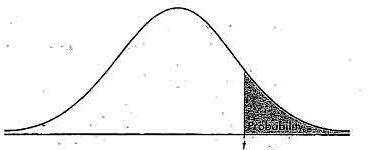
\includegraphics[width=0.8\textwidth]{img/ttest1.jpeg}
			\begin{itemize}
				\item Symmetrical.
				\item \textbf{\color{airforceblue}Significance level}:
				      \begin{itemize}
					      \item E.g., $\text{sig} = 0.05$ or $5\%$ means $M_1$ \& $M_2$ are significantly different for $95\%$ of population.
				      \end{itemize}
				\item Confidence limit: $z = \frac{\text{sig}}{2}$.
			\end{itemize}
		\end{column}
		\begin{column}{0.5\textwidth}
			\centering
			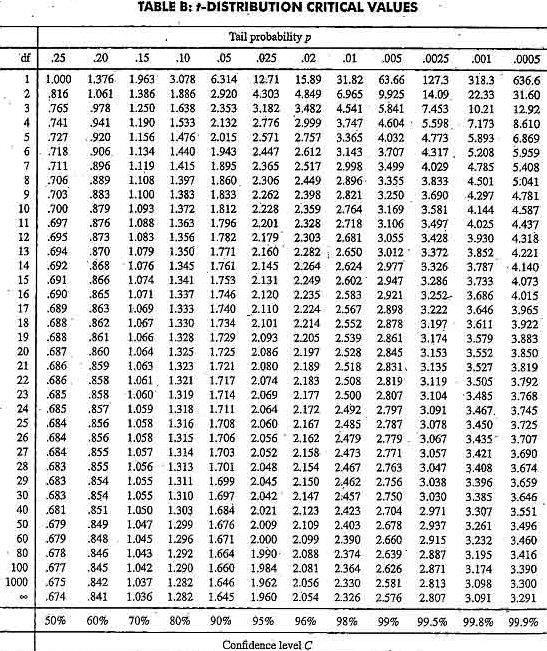
\includegraphics[width=0.7\textwidth]{img/ttest2.jpeg}
		\end{column}
		% TODO: Recreate plot in tikz.
	\end{columns}
\end{frame}

\begin{frame}{Estimating Confidence Intervals: Statistical Significance}
	\textbf{Are $M_1$ and $M_2$ {\color{airforceblue} significantly different}?}
	\begin{itemize}
		\item Compute $t$. Select significance level (E.g., sig = $5 \%$).
		\item Consult table for $t$-distribution:
		      \begin{itemize}
			      \item $t$-distribution is symmetrical:
			            \begin{itemize}
				            \item Typically upper $\%$ points of distribution shown.
			            \end{itemize}
			      \item Find critical value $c$ corresponding to $k-1$ degrees of freedom (here, $9$)
			      \item and for confidence limit $z = \frac{\text{sig}}{2}$ (here, $0.025$).
			      \item $\implies$ Here, critical value $c = 2.262$
		      \end{itemize}
		\item If $t > c$ or $t < -c$, then $t$ value lies in rejection region:
		      \begin{itemize}
			      \item \textbf{Reject null hypothesis} that mean error rates of $M_1$ and $M_2$ are equal.
			      \item Conclude: \textbf{statistically significant difference} between $M_1$ and $M_2$.
		      \end{itemize}
		\item Otherwise, conclude that any difference is chance.
	\end{itemize}
\end{frame}

\begin{frame}{Model Selection: Receiver Operating Characteristics (ROC) Curves}
	\vspace*{-1.5em}
	\begin{columns}
		\begin{column}{0.6\textwidth}
			\begin{itemize}
				\item Visual comparison of classification models.
				\item Compares and shows \textit{trade-off} between TPR and FPR:
				      \begin{itemize}
					      \item True Positive Rate (\textbf{TPR}): Proportion of positive tuples correctly classified as positive.\\
					            $\rightarrow$ sensitivity or recall $= \frac{\text{TP}}{\text{P}}$
					      \item False Positive Rate (\textbf{FPR}:) Proportion of negative tuples correctly classified as negative.\\
					            $\rightarrow \text{FPR} = \frac{\text{FP}}{\text{N}} = 1 - \text{Specificity}$
				      \end{itemize}

				\item \textbf{The area under the ROC curve is a
						      {\color{airforceblue}measure of the accuracy} of the model.}
				      Maximum area of $1.0$ for a perfect classifier.
				\item \textbf{The closer to the diagonal line (i.e. the closer the
					      area is to $0.5$), the less accurate is the model.}

			\end{itemize}
		\end{column}
		\begin{column}{0.4\textwidth}
			\vspace*{-1.5em}
			\begin{figure}
				\centering
				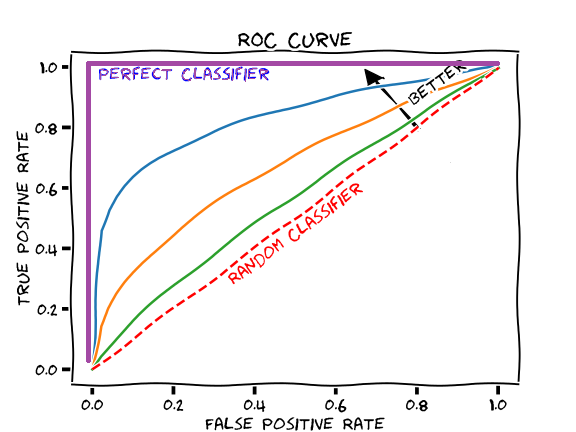
\includegraphics[width=\textwidth]{img/roc-curve.png}
			\end{figure}
			\vspace*{-0.5em}
			\scriptsize
			How to draw: Order tuples in decreasing order of probability.
			\begin{itemize}
				\item If TP move up TPR and plot point.
				\item If negative tuple classified as positive: move both FPR and FPR.
			\end{itemize}
		\end{column}
	\end{columns}
\end{frame}

\begin{frame}{Other Aspects of Model Selection}
	\begin{itemize}
		\item \textbf{Speed}
		      \begin{itemize}
			      \item Computational cost to train a classifier.
			      \item Time to use model (prediction time).
		      \end{itemize}
		\item \textbf{Robustness}, i. e. the ability to make accurate predictions.
		      \begin{itemize}
			      \item Noisy data.
			      \item Missing values.
		      \end{itemize}
		\item \textbf{Scalability}, i . e. efficient construction of classifiers on an abundant amount of training tuples.
		\item \textbf{Interpretability}, refers to understanding and insight
		      \begin{itemize}
			      \item Typically subjective and difficult to access.
			      \item Decision trees and classification rules are easy to interpret, but interpretability degrades with the size.
		      \end{itemize}
		\item \textit{Other measures} such as goodness of rules, decision-tree size or compactness of classification rules.
	\end{itemize}
\end{frame}

\section{Ensemble Methods: Increasing the Accuracy}

\begin{frame}{Ensemble Methods: Increasing the Accuracy}
	\begin{columns}
		\begin{column}{0.4\textwidth}
			\centering
			\begin{itemize}
				\item \textbf{{\color{airforceblue}Ensemble} methods:}
				      \begin{itemize}
					      \item Use a combination of models to increase accuracy.
					      \item Combine a series of $k$ learned models, $M_1$, $M_2$, $\ldots$, $M_k$, with the aim of creating an improved model $M^*$.
				      \end{itemize}
			\end{itemize}
		\end{column}
		\begin{column}{0.5\textwidth}
			\centering
			\begin{itemize}
				\item \textbf{Popular ensemble methods:}
				      \begin{itemize}
					      \item Bagging:
					            \begin{itemize}
						            \item Averaging the prediction over a collection of classifiers.
					            \end{itemize}
					      \item Boosting:
					            \begin{itemize}
						            \item Weighted vote with a collection of classifiers.
					            \end{itemize}
					      \item Ensemble:
					            \begin{itemize}
						            \item Combining a set of heterogeneous classifiers.
					            \end{itemize}
				      \end{itemize}
			\end{itemize}
		\end{column}
	\end{columns}
\end{frame}

\begin{frame}{Bagging: Boostrap Aggregation}
	\begin{itemize}
		\item \textbf{Analogy:}
		      \begin{itemize}
			      \item Diagnosis based on multiple doctors' majority vote.
		      \end{itemize}
		\item \textbf{Training:}
		      \begin{itemize}
			      \item Given a set $D$ of d tuples, at each iteration $i$, a training set $D_i$ of $d$ tuples is sampled with replacement from $D$ (i.e., bootstrap).
			      \item A classifier model $M_i$ is learned for each training set $D_i$.
		      \end{itemize}
		\item \textbf{Classification: classify an unknown sample $X$.}
		      \begin{itemize}
			      \item Each classifier $M_i$ returns its class prediction.
			      \item The bagged classifier $M^*$ counts the votes and assigns the class with the most votes to $X$.
		      \end{itemize}
		\item \textbf{Prediction:}
		      \begin{itemize}
			      \item Can be applied to the prediction of continuous values by taking the average value of each prediction for a given test tuple.
		      \end{itemize}
		\item \textbf{Accuracy:}
		      \begin{itemize}
			      \item Often significantly better than a single classifier derived from $D$.
			      \item For noisy data: not considerably worse, more robust.
			      \item Proved improved accuracy in prediction.
		      \end{itemize}
	\end{itemize}
\end{frame}

\begin{frame}{Boosting}
	\begin{itemize}
		\item \textbf{Analogy:}
		      \begin{itemize}
			      \item Consult several doctors, based on a combination of weighted diagnoses -- weight assigned based on the previous diagnosis accuracy
		      \end{itemize}
		\item \textbf{How boosting works:}
		      \begin{itemize}
			      \item Weights are assigned to each training tuple.
			      \item A series of $k$ classifiers is iteratively learned.
			      \item After a classifier $M_i$ is learned, the weights are updated to allow the subsequent classifier, $M_{i+1}$ to pay more attention to the training tuples that were misclassified by $M_i$.
			      \item The final $M^*$ combines the votes of each individual classifier, where the weight of each classifier's vote is a function of its accuracy.
		      \end{itemize}
		\item \textbf{Boosting algorithm can be extended for numeric prediction.}
		      \begin{itemize}
			      \item Each classifier $M_i$ returns its class prediction.
			      \item The bagged classifier $M^*$ counts the votes and assigns the class with the most votes to $X$.
		      \end{itemize}
	\end{itemize}
\end{frame}

\begin{frame}{AdaBoost ("Adaptive Boosting" (Freund and Schapire, 1997))}
	\begin{itemize}
		\item \textbf{Given a set of d class-labeled tuples: $(x_1 , y_1), \ldots, (x_d, y_d)$.}
		\item \textbf{Initially, all the weights of tuples are set the same: $\frac{1}{d}$.}
		\item \textbf{Generate $k$ classifiers in $k$ rounds. At round $i$,}
		      \begin{itemize}
			      \item Tuples from $D$ are sampled (with replacement) to form a training set $D_i$ of the same size.
			      \item Each tuple's chance of being selected is based on its weight.
			      \item A classification model $M_i$ is derived from $D_i$.
			      \item Its error rate is calculated using $D_i$ as a test set.
			      \item If a tuple is misclassified, its weight is increased, otherwise it is decreased.
		      \end{itemize}
		\item \textbf{Error rate: $\text{err}(x_j)$ is the misclassification error of tuple $x_j$. Classifier $M_i$ error rate is the sum of the weights of the misclassified tuples:}
		      \begin{align}
			      \text{error}(M_i) = \sum_{j=1}^{d} w_j \cdot \text{err}(x_j).
		      \end{align}
		      \textbf{The weight of classifier $M_i$'s vote is: $\log \frac{1-\text{error}(M_i)}{\text{error}(M_i)}$.}
	\end{itemize}
\end{frame}

\begin{frame}{Random Forest (Breiman, 2001)}
	\begin{itemize}
		\item \textbf{Random forest:}
		      \begin{itemize}
			      \item Each classifier in the ensemble is a decision-tree classifier and is generated using a random selection of attributes at each node to determine the split.
			      \item During classification, each tree votes and the most popular class is returned.
		      \end{itemize}
		\item \textbf{Two methods to construct random forests:}
		      \begin{itemize}
			      \item Forest-RI (random input selection):
			            \begin{itemize}
				            \item Randomly select, at each node, F attributes as candidates for the split at the node. The CART methodology is used to grow the trees to maximum size.
			            \end{itemize}
			      \item Creates new attributes (or features) that are a linear combination of the existing attributes (reduces the correlation between individual classifiers).
		      \end{itemize}
		\item \textbf{Comparable in accuracy to AdaBoost, but more robust to errors and outliers.}
		\item \textbf{Insensitive to the number of attributes selected for consideration at each split, and faster than bagging or boosting.}
	\end{itemize}
\end{frame}

\begin{frame}{Classification of Class-imbalanced Data Sets}
	\begin{itemize}
		\item \textbf{Class-imbalance problem:}
		      \begin{itemize}
			      \item Rare positive example but numerous negative ones.
			            \begin{itemize}
				            \item E.g., medical diagnosis, fraud, oil-spill, fault, etc.
			            \end{itemize}
			      \item Traditional methods assume a balanced distribution of classes and equal error costs: not suitable for class-imbalanced data.
		      \end{itemize}
		\item \textbf{Typical methods for imbalanced data in 2-class classification:}
		      \begin{itemize}
			      \item \textbf{\color{airforceblue}Oversampling:}
			            \begin{itemize}
				            \item Re-sampling of data from positive class.
			            \end{itemize}
			      \item \textbf{\color{airforceblue}Undersampling:}
			            \begin{itemize}
				            \item Randomly eliminate tuples from negative class.
			            \end{itemize}
			      \item \textbf{\color{airforceblue}Threshold-moving:}
			            \begin{itemize}
				            \item Moves the decision threshold, $t$, so that the rare-class tuples are easier to classify, and hence, less chance of costly false-negative errors
			            \end{itemize}
			      \item \textbf{\color{airforceblue}Ensemble techniques:}
			            \begin{itemize}
				            \item Ensemble multiple classifiers introduced above.
			            \end{itemize}
		      \end{itemize}
		\item \textbf{Still difficult on multi-class tasks.}
	\end{itemize}
\end{frame}

\section{Summary}

\begin{frame}{Summary}
	\begin{itemize}
		\item \textbf{Classification.}
		      \begin{itemize}
			      \item A form of data analysis that extracts models describing important data classes.
		      \end{itemize}
		\item \textbf{Effective and scalable methods devopeped for:}
		      \begin{itemize}
			      \item Decision-tree induction, naive Bayesian classification, rule-based classification, and many other classification methods.
		      \end{itemize}
		\item \textbf{Evaluation metrics:}
		      \begin{itemize}
			      \item Accuracy, sensitivity, specificity, precision, recall, $F$-measure, and $F_\beta$-measure.
		      \end{itemize}
		\item \textbf{Stratified $k$-fold cross-validation.}
		      \begin{itemize}
			      \item Recommended for accuracy estimation.
		      \end{itemize}
		\item \textbf{Significance tests and ROC curves.}
		      \begin{itemize}
			      \item Useful for model selection.
		      \end{itemize}
	\end{itemize}
\end{frame}

\begin{frame}[c]
  \begin{center}
    {\bf Any questions about this chapter?}\\[0.5cm]
    Ask them now or drop us a line: \\\bigskip
    Dominik Probst\\
    \faPaperPlane[regular] \ \texttt{dominik.probst@fau.de}\\\smallskip
    \&\\\smallskip
    Melanie B. Sigl\\
    \faPaperPlane[regular] \ \texttt{melanie.sigl@fau.de}.
  \end{center}
\end{frame}
\section{Appendix}
\appendix
\begin{frame}{\vspace*{-2em}Basic Decision Tree Algorithm}\label{algo:decision-tree}
	\vspace*{-2em}
	\scriptsize
	\begin{algorithm}[H]
		\caption{\texttt{build\_decision\_tree}. Generate a decision tree from training tuples in data partition $D$.}
		\SetAlgoVlined
		\begin{multicols}{2}
			\KwData{
				\begin{itemize}
					\item Training dataset $D$ containing tuples with their associated class labels;
					\item \texttt{attribute\_list}, the set of candidate attributes;
					\item \texttt{attribute\_selection\_method}, a method to determine the splitting criterion that ``best'' partitions the data tuples into individual classes. The criterion consists of a \texttt{splitting\_attribute}, and possibly, either a \texttt{split\_point} or \texttt{splitting\_subset}.
				\end{itemize}
			}
			\KwResult{A decision tree.}
			\BlankLine
			create a node $N$\;
			\If{tuples in $D$ are all of the same class $C$}{
				\KwRet{
					$N$ as a leaf node labeled with the class $C$\;
				}
			}
			\If{\texttt{attribute\_list} is empty}{
				\tcc{Majority voting}
				\texttt{majority\_class} $\leftarrow$ determine majority class in $D$\;
				\KwRet{
					$N$ as a leaf node labeled with \texttt{majority\_class}\;
				}
			}
			\tcc{apply \texttt{attribute\_selection\_method} to find the ``best'' \texttt{splitting\_criterion}}
			\texttt{splitting\_criterion} $\leftarrow$ \texttt{attribute\_selection\_method}($D$, \texttt{attribute\_list})\;
			label node $N$ with \texttt{splitting\_criterion}\;

			\If{(\texttt{splitting\_attribute} is discrete-valued \textbf{and} multiway splits allowed) \textbf{or} attribute value has only one unique value}{
				\tcp{remove \texttt{splitting\_attribute}}
				\texttt{attribute\_list} $\leftarrow$ \texttt{attribute\_list} - \texttt{splitting\_attribute}\;

			}
			\ForEach{outcome $j$ of \texttt{splitting\_criterion}}{
				\tcc{partition the tuples and grow subtrees for each partition}
				$D_j$ $\leftarrow$ partition $D$ to satisfy outcome $j$\;
				\If{$D_j$ is empty}{
					attach a leaf labeled with the majority class in $D$ to node $N$\;
				}
				\Else{
					attach the node return by \texttt{build\_decision\_tree}($D_j$, \texttt{attribute\_list}) to node $N$\;
				}
			}
			\BlankLine
			\KwRet{
				$N$\;
			}
		\end{multicols}
	\end{algorithm}
\end{frame}


\end{document}
